% This is "sig-alternate.tex" V2.1 April 2013
% This file should be compiled with V2.5 of "sig-alternate.cls" May 2012
%
% This example file demonstrates the use of the 'sig-alternate.cls'
% V2.5 LaTeX2e document class file. It is for those submitting
% articles to ACM Conference Proceedings WHO DO NOT WISH TO
% STRICTLY ADHERE TO THE SIGS (PUBS-BOARD-ENDORSED) STYLE.
% The 'sig-alternate.cls' file will produce a similar-looking,
% albeit, 'tighter' paper resulting in, invariably, fewer pages.
%
% ----------------------------------------------------------------------------------------------------------------
% This .tex file (and associated .cls V2.5) produces:
%       1) The Permission Statement
%       2) The Conference (location) Info information
%       3) The Copyright Line with ACM data
%       4) NO page numbers
%
% as against the acm_proc_article-sp.cls file which
% DOES NOT produce 1) thru' 3) above.
%
% Using 'sig-alternate.cls' you have control, however, from within
% the source .tex file, over both the CopyrightYear
% (defaulted to 200X) and the ACM Copyright Data
% (defaulted to X-XXXXX-XX-X/XX/XX).
% e.g.
% \CopyrightYear{2007} will cause 2007 to appear in the copyright line.
% \crdata{0-12345-67-8/90/12} will cause 0-12345-67-8/90/12 to appear in the copyright line.
%
% ---------------------------------------------------------------------------------------------------------------
% This .tex source is an example which *does* use
% the .bib file (from which the .bbl file % is produced).
% REMEMBER HOWEVER: After having produced the .bbl file,
% and prior to final submission, you *NEED* to 'insert'
% your .bbl file into your source .tex file so as to provide
% ONE 'self-contained' source file.
%
% ================= IF YOU HAVE QUESTIONS =======================
% Questions regarding the SIGS styles, SIGS policies and
% procedures, Conferences etc. should be sent to
% Adrienne Griscti (griscti@acm.org)
%
% Technical questions _only_ to
% Gerald Murray (murray@hq.acm.org)
% ===============================================================
%
% For tracking purposes - this is V2.0 - May 2012

\documentclass{vldb}
\usepackage{lipsum}% http://ctan.org/pkg/lipsum
\usepackage{graphicx}% http://ctan.org/pkg/graphicx
\usepackage{float}
\usepackage{todonotes}
\usepackage{color}
\usepackage[outdir=./figures/]{epstopdf}
\usepackage{listings}
\usepackage{subcaption}
\usepackage[blocks]{authblk}
\begin{document}
%\lstset{numbers=left, numberstyle=\small, numbersep=8pt, frame = single, language=Pascal, framexleftmargin=15pt}





%
% --- Author Metadata here ---
%\conferenceinfo{WOODSTOCK}{'97 El Paso, Texas USA}
%\CopyrightYear{2007} % Allows default copyright year (20XX) to be over-ridden - IF NEED BE.
%\crdata{0-12345-67-8/90/01}  % Allows default copyright data (0-89791-88-6/97/05) to be over-ridden - IF NEED BE.
% --- End of Author Metadata ---

\title{Continuous Training of Large Scale Machine Learning Models}

%
% You need the command \numberofauthors to handle the 'placement
% and alignment' of the authors beneath the title.
%
% For aesthetic reasons, we recommend 'three authors at a time'
% i.e. three 'name/affiliation blocks' be placed beneath the title.
%
% NOTE: You are NOT restricted in how many 'rows' of
% "name/affiliations" may appear. We just ask that you restrict
% the number of 'columns' to three.
%
% Because of the available 'opening page real-estate'
% we ask you to refrain from putting more than six authors
% (two rows with three columns) beneath the article title.
% More than six makes the first-page appear very cluttered indeed.
%
% Use the \alignauthor commands to handle the names
% and affiliations for an 'aesthetic maximum' of six authors.
% Add names, affiliations, addresses for
% the seventh etc. author(s) as the argument for the
% \additionalauthors command.
% These 'additional authors' will be output/set for you
% without further effort on your part as the last section in
% the body of your article BEFORE References or any 


\renewcommand\Authfont{\fontsize{13}{14.4}\selectfont \bfseries }
\renewcommand\Affilfont{\fontsize{10}{14.4}\selectfont \normalfont}

\author[1]{Behrouz Derakhshan}
\author[1,2]{Tilmann Rabl}
\author[1,2]{Volker Markl}

\affil[1]{DFKI, Germany \protect\\ \normalsize{firstname.lastname@dfki.de}}  

\affil[2]{TU Berlin, Germany \protect\\  \normalsize{firstname.lastname@tu-berlin.de}}



%\author{
%\alignauthor
%Behrouz Derakhshan\\
%	\email{behrouz.derakhshan@dfki.de}
%% 2nd. author
%\alignauthor
%Tilmann Rabl \\
%	\email{rabl@tu-berlin.de}
%% 3rd. author
%\alignauthor 
%Volker Markl\\
%	\email{volker.markl@tu-berlin.de}
%}

\maketitle
\begin{abstract}
\todo[inline]{first paragraph too long? get to the point faster}
%Volker
Many scientific and business applications rely on methods from machine learning in order to derive novel insight from large data sets.
%Volker
%Volker
A data analytics process is a pipeline comprised of several steps, from source selection, data preparation, feature engineering, model building/training, to the deployment of the model in a production environment. 
Many of these steps are not automated, but require manual configuration by a data scientist or are semi-automatic at best.
%Volker
Once a machine learning model is trained on an initial dataset it is deployed into a system where it can answer prediction queries in a realtime and reliable fashion.
When new training data becomes available while the system is running, the model is updated.
These updates are typically applied incrementally.
However, to ensure higher quality of prediction and better adoption to changes in data distribution, models are retrained.
Retraining of models is a time consuming and resource intensive process.

In this paper, we propose a novel deployment method for stochastic gradient descent (SGD)-based machine learning models.
SGD is an iterative process, which works well with large data sets.
During each iteration, SGD updates the model based on one or sample of the training items.
Using this property, we eliminate the need for complete retraining by replacing it with a series of consecutive SGD iterations.
We show that individual iterations of SGD are light weight and can be executed while the system is running.
Our experiments show that our deployment method updates models an order of magnitude faster, without degrading the quality of the model.
Furthermore, models can adopt faster to changes in data distribution using our deployment method.
\end{abstract}


\keywords{Machine Learning Model Management; Stochastic Gradient Descent; Machine Learning Systems}

\section{Introduction} \label{introduction}
\todo[inline]{POLISH}
\todo[inline]{Remove mentions of MNIST}
\todo[inline]{CRITEO Dataset experiments}
\todo[inline]{mention retraining points in the experiments}
\todo[inline]{Remove image classifier mention from conclusion}
\todo[inline]{Make sure there are no repetitions in the paper}
\todo[inline]{Add BBDC and streamline funding id}
\todo[inline]{improve based on Volker's comments}
% Problem
Deploying and maintaining machine learning (ML) models is a crucial step in the lifecycle of a machine learning application. 
%Volker
Despite the fact that deployment and serving of ML models puts learning into practice and thus is the aspect that provides the actual (business) value, it has received very little attention.
%Volker
% Specific problem
In order to sustain the performance of a model in a dynamic environment, where data and thus models may change, we have to monitor the performance of the model in realtime during its deployment and update the model when necessary.

However, Incremental updates alone are not enough to maintain model quality. 
When the data distribution changes quickly, the model will not adjust in a timely fashion. 
Furthermore, new batch datasets from external sources may become available while the system is running.
Lastly, incrementally updating may not arrive at the same quality of model as a complete batch training.
Therefore, in order to prevent the model's quality from degrading, periodic retraining should be performed to better fit the model with the data that has arrived at the system since the last training.

% How is it different from prior work
Most of the current machine learning research focuses on training and providing tools to make model training and search easier. 
Kumar et al. \cite{kumar2015survey} provided an overview of landscape of existing machine learning systems. 
Most of the surveyed systems focus on training of machine learning models and provide little to no support after the model has been trained.
Only few systems \cite{akdere2011case, crankshaw2014missing}, support deploying and maintaining the models as well.
Moreover, systems with support for model deployment are still lacking constant monitoring and fast and accurate updates of the machine learning models.
The whole process of training and deployment of models is usually performed manually.
\todo[inline]{move velox and continuous diagrams here}
The most common approach is as follows; first a model is trained based on an existing dataset residing on disk, this model serves as the initial model.
This model is then deployed to an environment where it can answer prediction queries arriving at the system.
The system also receives feedback in the form of new training observations.
Upon receiving a training observation, the model is updated incrementally.
Incremental updates are only supported by certain type of machine learning models, where the underlying optimization strategy allows the system to change the model based on individual training items.

\textbf{Example application:} to illustrate this model deployment approach, consider the task of predicting the click through rate (CTR) of online advertisements.
To maximize benefit, advertisement providers use machine learning models to estimate the expected click rate of different advertisements.
They train machine learning models based on the available data, which typically includes content of the page, search query, user information, content and meta-data of the available advertisements. 
Once the model is deployed, prediction queries of the form of ad requests arrive at the system.
The model displays the advertisements that have the highest probabilities of being clicked by the user.
Based on whether or not advertisements are clicked on, the system sends feedback in the form of new training observations and the model is updated accordingly.
Furthermore, new batch training datasets in the form of user databases, new advertisements with their metadata and more web pages will become available as more companies employ the service of the advertisement provider.
In order to leverage the new data and reduce the error introduced by incremental learning, the model is periodically retrained using entire data.
\todo[inline]{inconsistency, search engine provider, ad provider}
Figure \ref{fig:click-rate} demonstrates the CTR prediction use case for a search engine provider.

\begin{figure}[h]
\centering
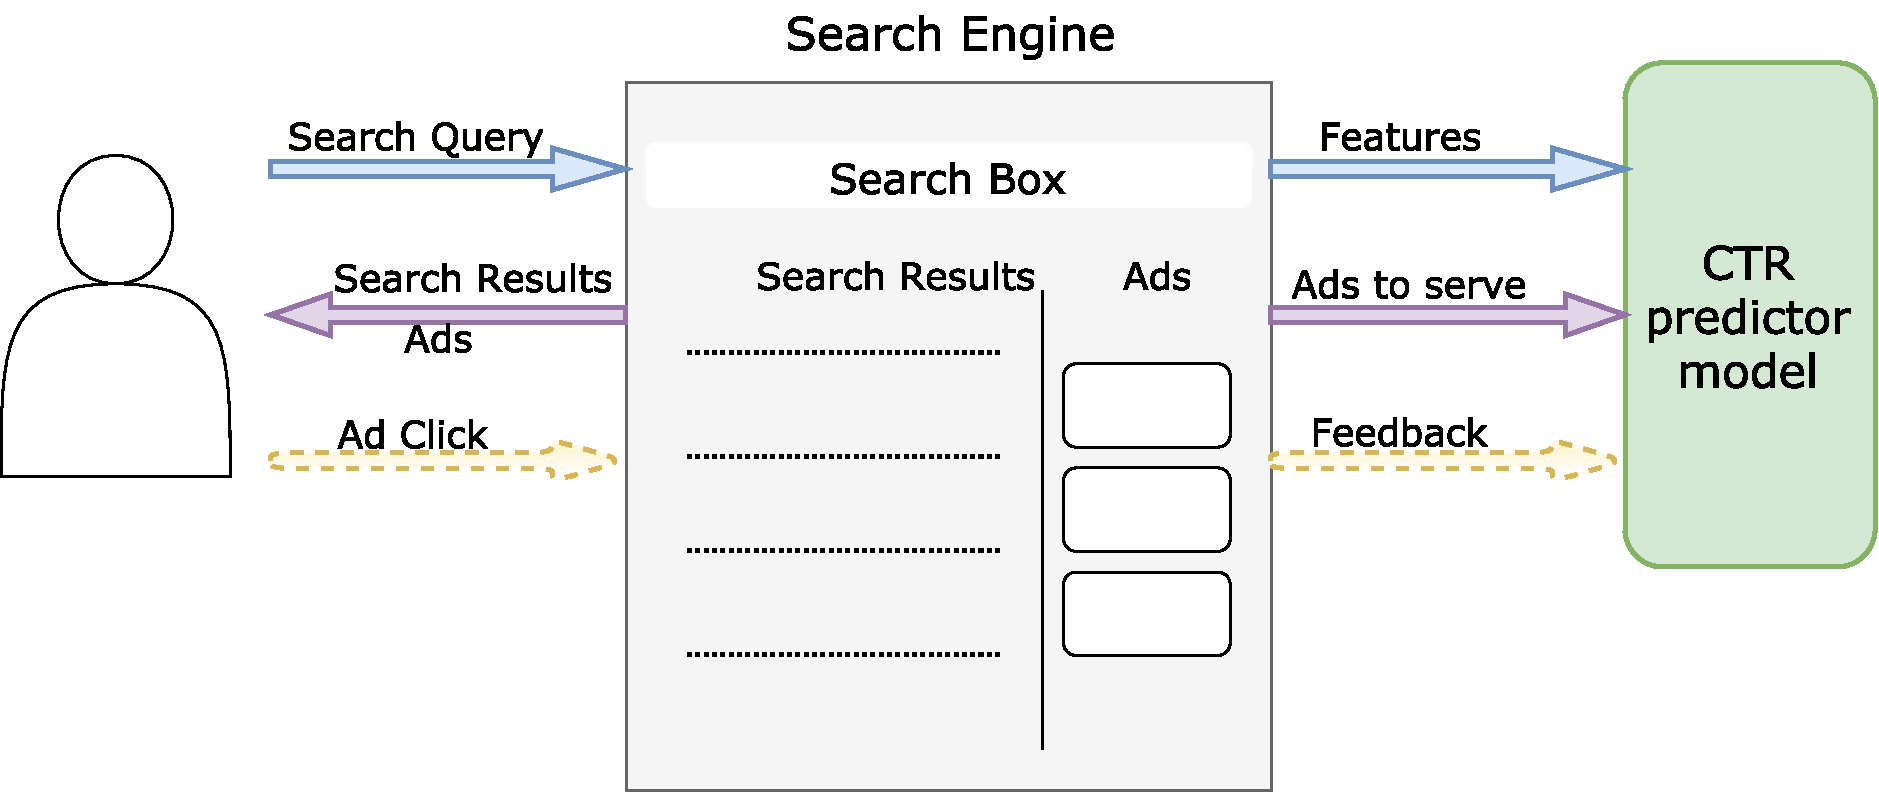
\includegraphics[width=\columnwidth]{../images/use-case-4.pdf}
\caption{Use Case: Click Through Rate Prediction}
\label{fig:click-rate}
\end{figure}

Some emerging machine learning systems have tried to automate this process \cite{crankshaw2014missing}.
They automatically deploy the model into a production environment, monitor its quality, and initiate a retraining when required.
However, they treat the underlying machine learning models as black boxes. 
As a result, they miss many opportunities for optimizing the training and deployment process.
% What is the motivation for this work
%Given the lack of systems to support model deployment and maintenance, we have set out to design a system that not only supports deployment and maintenance of machine learning models but also provides %constant crashing and batch updates while the system is running. 
%We propose the design of a system that provide 
%real-time query support as well incremental and fast batch updates to the machine learning models.

Our key observation is that, by exploiting the iterative nature of the underlying optimization algorithm (stochastic gradient descent), the model training process can be seamlessly executed with the serving and query answering component.
Based on this observation, we present a new model for a system, that supports deployment, maintenance, and incremental and fast batch updates of machine learning models.
We are making the following contributions: 
\begin{itemize}
\item we define a system for machine learning models deployment and maintenance and provide a prototypical implementation
%Volker
\item we allow for incremental updates to the model, thus handling changes in the data distribution
%Volker
\item we eliminate offline batch retraining and replace it with a series of single iteration of SGD
\end{itemize}
%Volker
Our experiments show that our approach improves the runtime of model training and deployment by an order of magnitude over the state of the art while retaining the quality of the model. 
%Volker
This is due to the fact that we are able to completely eliminate batch retraining. 
Our method can also adapt to changes in the distribution faster than the existing methods.

% Outline: The rest of this document is structured as follows. ...
The rest of this paper is organized as follows. 
Section \ref{sgd} describes the underlying optimization method.
Section \ref{continious-training-serving} introduces the design principles of our system. 
Section \ref{sec:system-architecutre} discusses the architecture and components.
In Section \ref{evaluation}, we evaluate our system against different workloads and compare the performance of our method to other model deployment and maintenance approaches. 
Section \ref {related-work} discusses related work.
Finally, Section \ref{conclusion} presents our conclusion and future work.

\section{Stochastic Gradient Descent} \label{sgd}
Machine learning applies optimization methods in order to find the minimum of an objective function (referred to as the loss function) by calculating the gradient of the function at different data points and update the function parameters based on the gradient values.
A common optimization method is gradient descent, an iterative process where in every iteration the entire training data set is used to calculate the gradient value.
One drawback of gradient descent is that in presence of large datasets it will become very slow since every iteration has to inspect all the training items.
Stochastic gradient descent (SGD) \cite{bottou2010large} is an approximation of the gradient descent method. 
Similar to gradient descent, it is an iterative process but in each iteration it operates on one element (or a sample of elements) at a time. 
It calculates the gradient at a single element and updates the parameters of the model accordingly. 
Although it converges after a higher number of iterations, the overall convergence time is lower (sometimes by orders of magnitude) than gradient descent. 
Each iteration of SGD can be executed in a short amount of time since it only works with a sample of the data.
We are leveraging this property of SGD and design our deployment system so that it executes one iteration of SGD at a time without interrupting the query answering component.
In Section \ref{evaluation} we show that the time to execute a single iteration of SGD is insignificant.

\subsection{Distributed SGD}
To efficiently train machine learning models on large datasets, scalable techniques have to be employed.
As explained earlier, SGD inherently works well with large amount of data since it does not need to scan every data point during every iteration.
However, the problem arises when the dataset cannot fit into the memory of a single machine and has to be distributed.
In this situation, one common method is to distribute the gradient calculation tasks across the nodes in the cluster, where each task will work with a different part of the data.
One problem of this approach is that a synchronization step is required before applying the updates to the model. 
This synchronization step slows down the SGD process, because after every iteration, all the updates have to be sent to a central process that updates the model.
Experiments on distributed, asynchronous SGD \cite{recht2011hogwild, dean2012large} show that the quality of the final model is not any worse than the synchronized approach. 

\subsection{Learning Rate Tuning} \label{learning-rate}
Learning rate or step size is a parameter of SGD, which controls the amount of change in model parameters during each iteration of SGD.
It plays an important role in the convergence of SGD.
The most common technique is to set the learning rate to a small value, and slowly decrease the value in every iteration until the model converges.
However, in continuous and online learning due to possible changes in data distribution model's parameters may never converge.
Adaptive learning rates have been used in online scenarios where based on different criteria the learning rate is adjusted automatically.
Schaul et al. \cite{schaul2013no} have proposed one such method were the learning rate can be inferred automatically based on the changes in the parameters of the model. 
One advantage of their method is that it works well with non-stationary problems, where the distribution of the data is constantly changing. 
Based on observed changes in the data, one can adjust the learning rate to decrease (when approaching the optimum value) or increase (when the distribution of the data has changed).

\subsection{Machine Learning Models based on SGD}
SGD is one of the most common optimization methods for training machine learning models on large datasets. 
It has been used in classification \cite{zhang2004solving}, clustering \cite{bottou1995convergence}, neural networks \cite{dean2012large}, and matrix factorization \cite{funk2006netflix}.
Some examples of machine learning models that use SGD are: 

\textbf{Linear Classifiers} are arguably the most common type of machine learning models built using the SGD optimization method. 
In our CTR prediction example described in section \ref{introduction}, logistic regression method is used to train models for predicting the click through rate \cite{macmahan2013}. 
Logistic regression models typically output a probability instead of a class label \cite{hosmer2013applied} that indicates how likely an item belongs to a specific class.
In our example, for every available advertisement, the click probability is predicted and depending on how many advertisements will be displayed, the ones with highest probabilities are selected.
Support vector machine (SVM) \cite{steinwart2008support} is another common classification model.
While logistic regression model aims to find parameters of a function that accurately fit the data points to the labels, SVM tries to find a hyperplane that separates the data points belonging to different classes.
In many cases, both type of models work equally well, but depending the data and its complexity one method may be preferred to the other.

\textbf{Matrix Factorization} is a common method used in recommender systems \cite{koren2009matrix}. 
Matrix factorization is used to derive the latent factors (users and items) for recommender systems.
It relies on the fact that each user and item can be described in a few dimensions (10 to 40 usually) based on the available ratings.
These latent factors have automatically capture the similarity of users and items based on the ratings provided by the users.
Any unknown rating, hence can be predicted by simply using a dot product of the user vector with item vector.
A scalable version of the algorithm was proposed by Gemulla et al. \cite{gemulla2011large}.

\textbf{Neural Networks} or deep learning inspired by biological neural networks in brain are used to learn and approximate complex functions. 
They have been used for more than half a century to model functions and have been used in training machine learning models.
However, due to slow training process and lack of large amount of training data they have not been used extensively in machine learning community.
Past decade saw a change with publication of several nominal works.
Hinton et al. \cite{hinton2006fast} proposed methods for speeding up the training of neural networks.
ImageNet competition \cite{ILSVRC15} in 2012 was won by a neural network proposed by Krizhevsky et al. \cite{krizhevsky2012imagenet} where they significantly reduced the error rate. 
Success of Google Brain team \cite{sutskever2014sequence, mikolov2013efficient} was also instrumental to popularizing neural networks in machine learning community.
SGD is the idea optimization algorithm for training neural networks since it works very well with large datasets (which are required for training neural networks).
In fact, almost all of the recent works on neural networks use SGD for training them.
\begin{figure*}[t]
\centering
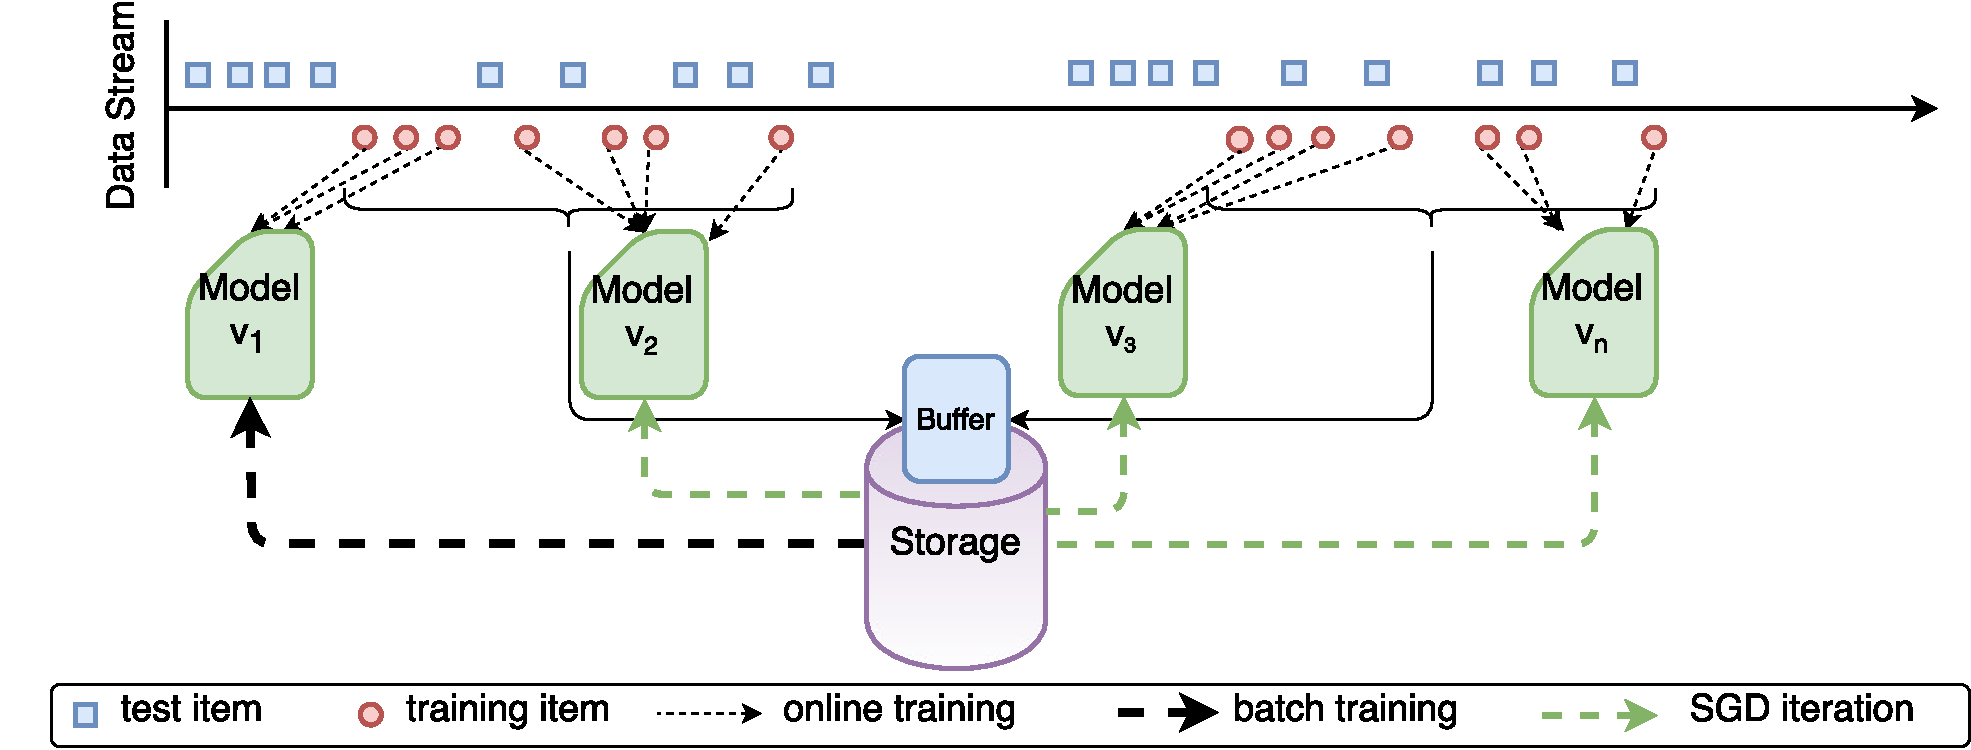
\includegraphics[scale = 0.5]{../images/continuous-1.pdf}
\caption{Continuous Training and Serving}
\label{fig:cont-training-serving}
\end{figure*}

\section{Continuous Training and Serving} \label{continious-training-serving}
% Stochastic Gradient System properties
%As described in Section \ref{sgd}, stochastic gradient descent is an iterative process where in each iteration one or a sample of the data is selected randomly and the gradient is calculated based on this sample. 
%After each iteration the parameters of the model are updated.
%As more iterations are executed, the model becomes more accurate.
%Since SGD can train a model using both individual and (mini-)batches of data items, it is an idea optimization methods for deployment environments.
%Initial models can be trained over large batches data.
%After the initial training, these models can be deployed into a production environment where they will answer prediction queries arriving at the system.
%As mentioned in section \ref{introduction} most systems incorporate a feedback mechanism where more training items will become available over time.
%With arrival of each new training item, SGD can incrementally update the model.
%In our CTR use case, initial training is performed over the available click behavior of the users.
%This data is gathered over a long period of time by observing what ads have been click by each specific users.
%After the model is deployed, prediction queries that contains users' and requested pages' information are send to the model.
%Based on this data and the properties of the available ads creatives, the model proposes the best set of ads to be shown to the user.
%The system collects feedback based on whether the user clicked on any of the given set of ads.
%If an ad is click by a user, this information is sent back to the system as a new training item which will be used to incrementally update the model.
%However, if an ad is not clicked by a user, it is not a strong indication of user's negative taste towards a specific ad.
%Therefore, training items with negative labels are typically only generated if an ad has a very low (close to zero) click ratio for a very long period of time.
%Our key observation is that, by utilizing SGD's properties, the model training process can be seamlessly executed along side the serving and query answering component.
%Similar to Velox, models are incrementally updated.
%However, unlike Velox, the retraining process is completely eliminated and instead is replaced by a series of consecutive 1-iteration of SGD optimization.
%Since each iteration of SGD is light and fast, it can be executed while the system is serving prediction requests.
Our proposed deployment and maintenance system uses SGD as its underlying learning algorithm.
As a result, it can update the model incrementally (one training item at a time) or use mini-batches of data (1 iteration of SGD).
The core design principles of our deployment system are threefold.
First, we incrementally update the model so that it can adapt to changes in the distribution of the incoming data.
Second, we eliminate retraining and replace it with a series of consecutive iterations of SGD.
And finally, we immediately use new batch datasets that are available to the system.
Figure \ref{fig:cont-training-serving} shows how our proposed deployment method works.
First, using the existing data residing on disk, we train an initial model and deploy it into the system.
The system receives prediction queries and training observations in a streaming fashion.
The deployed model answers incoming prediction queries as soon as they are received.
Once the system receives a training observation it updates the model incrementally.
The system also keeps track of incoming training observations and adds them to an intermediate buffer.
A scheduler component, will schedule a new iteration of SGD based on the rate of incoming training observations. 
The scheduler can also decide to run an iteration when the system is not under heavy load.
Each new iteration uses a random sample of the data in storage and the data in the buffer. 
Moreover, our system stores new batch datasets in the buffer (or persistent storage unit) as soon as they become available.
Any new scheduled iteration of SGD uses the newly introduced dataset to further train the model without requiring a new model to be retrained from scratch.

%\subsection{State of the Art} \label{sub:state-of-the-art}
%Velox \cite{crankshaw2014missing} is an state of the art system which has implemented this deployment model.
%It uses Apache Spark to train an initial model using the available training data.
%Once the model is trained, it is deployed into a distributed environment, where prediction queries are answered in real time.
%When new training data arrives at the system the model is incrementally updated.
%The incoming training data is also stored in a persistent storage.
%To ensure the model is performing well, its quality is monitored over time.
%Velox periodically retrains the model from scratch. 
%This retraining can be triggered when the size of new training data has surpasses a predefined limit, or the quality of the model has gone below a user defined threshold or simply after a fixed period of time defined by the user.
%Figure \ref{fig:velox-work-flow} depicts how Velox works. 
%A buffer is used to store the incoming training observations, which will be combined with the historical data during the next retraining phase.
%Although Velox continuously monitors and updates the underlying model, it has 3 drawbacks:\\
%\begin{itemize}
%\item Complete retraining discards all the current model parameter
%\item Process of retraining on full dataset is a time consuming process that requires a lot of resources
%\item When new datasets are introduced, a complete retraining has to be performed in order to update the model
%\end{itemize}
%While the model is being retrained, incremental updates are turned off.
%Moreover, newly introduced datasets will not have any effect on the model until the next retraining.
%This negatively affects the quality of the predictions produced by the system.
%To address these problems, we introduced a new deployment system which we describe next.

%\subsection{Continuous Deployment}


\section{System Architecture} \label{sec:system-architecutre}
\begin{figure}[t]
\centering
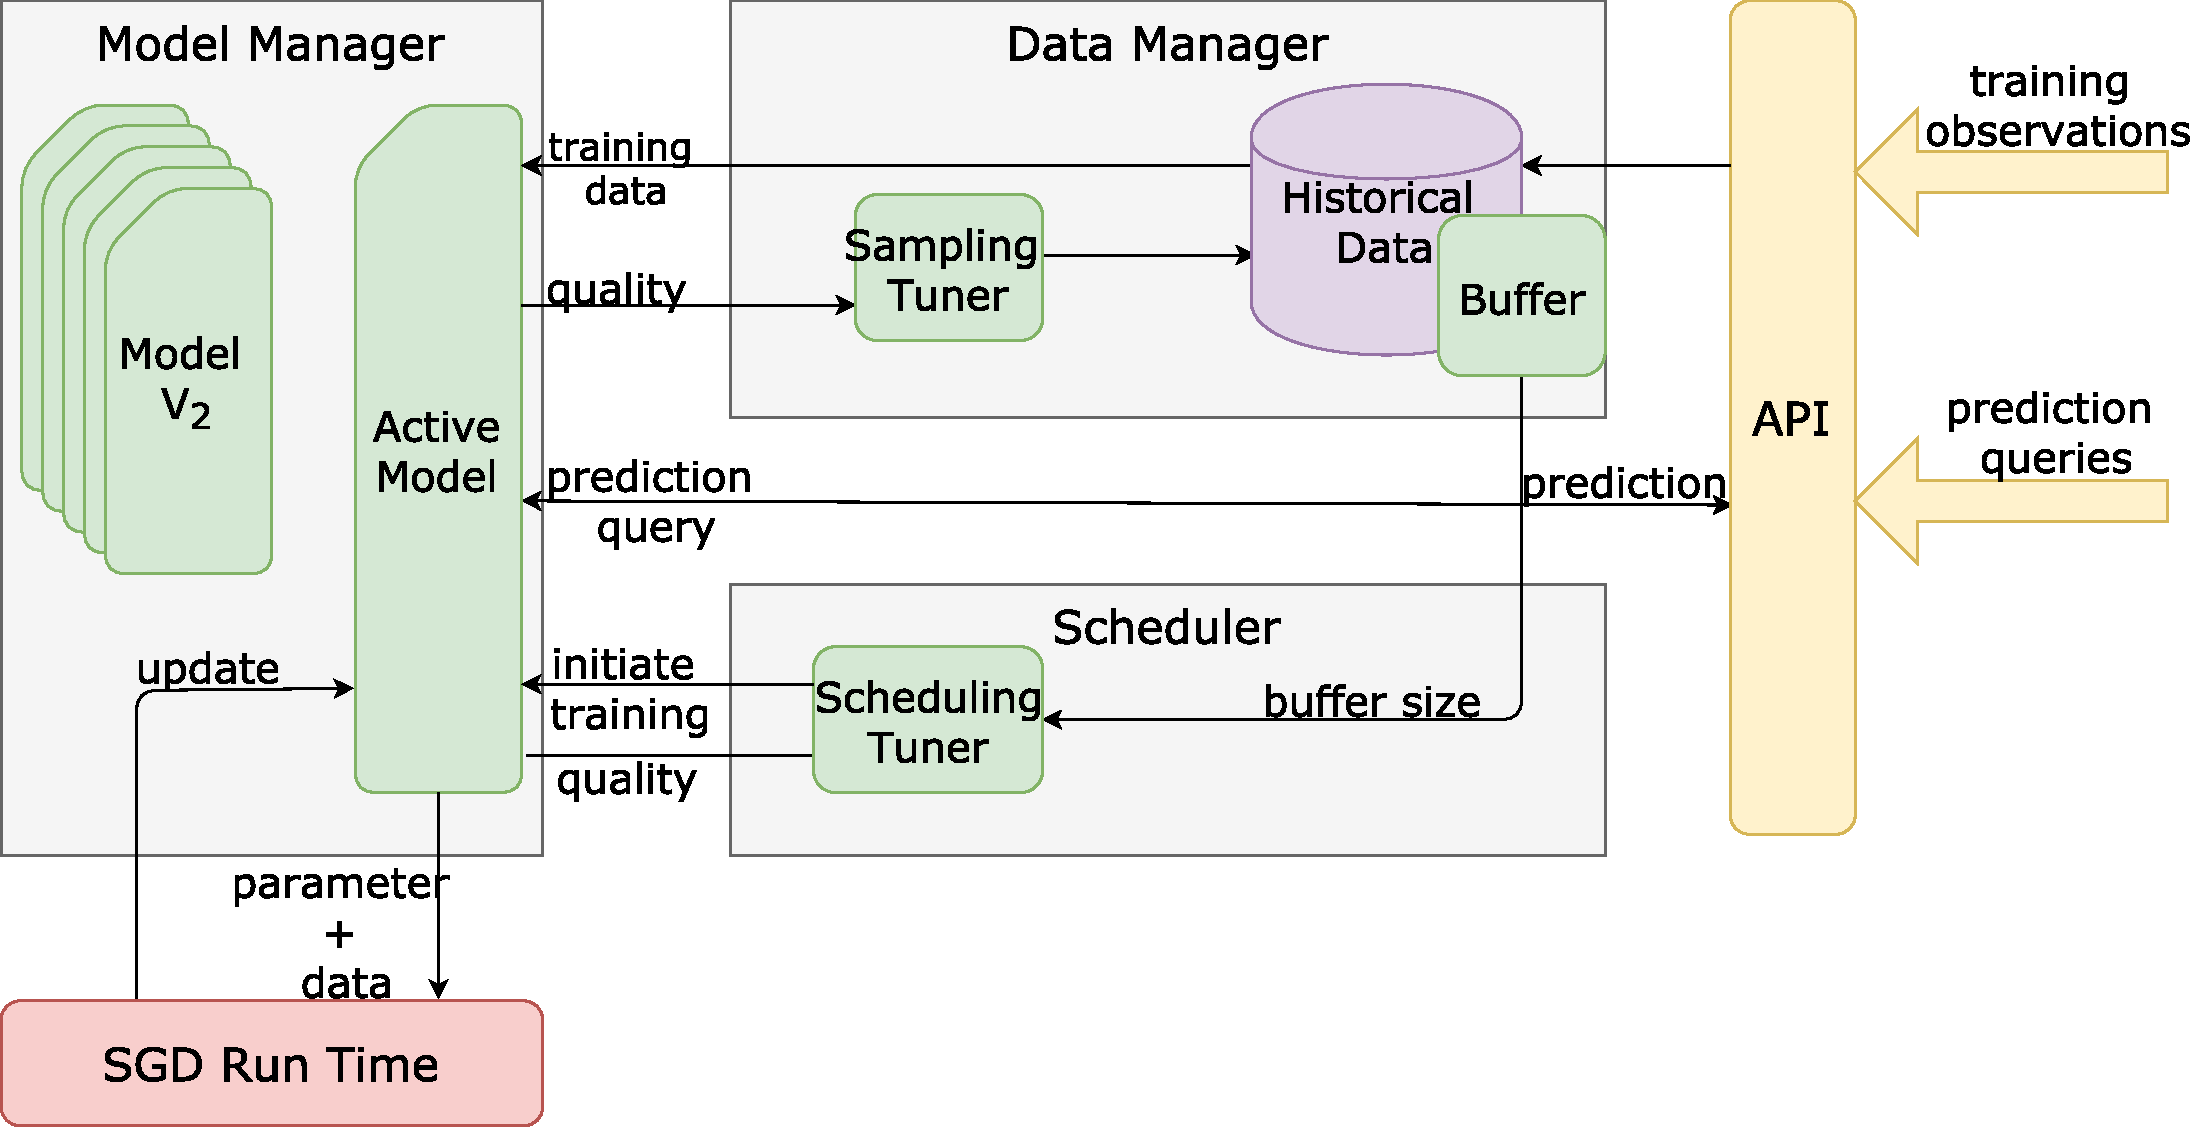
\includegraphics[width=\columnwidth]{../images/system-architecture-6.pdf}
\caption{System Architecture}
\label{fig:system-architecture}
\end{figure}
The proposed system comprises three main components; model manager, data manager and scheduler and an independent SGD run-time. 
Figure \ref{fig:system-architecture} gives an overview of the architecture of our system and the interactions between its components.
Incoming training observations are forwarded to the data manager.
The data manager first stores the training observations in a buffer and then passes them on to the model manager.
Model manager incrementally updates the model using the training observations.
Model manager is also responsible for receiving prediction requests.
Once it receives a request, it uses the latest version of the model to make a prediction and return the result to the user.
Both scheduler and data manager components are constantly communicating with each other and the model manager to obtain the latest statistics such as the model quality and buffer size, which in turn helps in tuning the scheduling and sampling rate for next iterations of SGD. 
Next, we explain each component of the system in more detail.

\subsection{Scheduler}\label{scheduler}
The scheduler component is responsible for scheduling of new iterations of SGD.
Intuitively, the best time to execute an iteration is when the system is not under heavy load.
This will help in utilizing the system's resources as well as keeping the model up to date at all time.
A new iteration of SGD should also be executed when the system receives more training data than can be handled by the intermediate buffer.
If the model is not updated with the new training items frequently, the quality will go down more rapidly, especially if the distribution of the data is changing.
In our prototype, the scheduling rate is controlled by a user defined parameter, \textit{max\_buffer\_size}.
When intermediate buffer's size reaches \textit{max\_buffer\_size}, the scheduler executes a new iteration of SGD.
It is important to note that the scheduling rate affects the quality of the model.
In Section \ref{evaluation}, we investigate the effect of scheduling rate on model quality.
If no new training data is available, the model parameters will eventually converge and any further training iterations will not have any effect on the model quality.
Therefore, the scheduler component has to communicate with the model manager in order to detect whether the model parameters have converged and stop further iterations until more training data becomes available.

\subsection{Data Manager} \label{data-manager}
In order to execute an iteration of SGD, we need to combine the training data that arrives at the system in real-time with the data stored on disk.
The data manager is responsible for storing the incoming training observations in an intermediate buffer.
When a new training iteration is scheduled, the data manager accesses the historical data stored on disk and provides a sample.
The data from the sample and the data in the buffer are merged together to create the dataset for next training iteration.
The data manager provides access to this dataset for model manager where the actual training and model updates happen.
The data manager also communicates with the scheduler in order to inform it when the intermediate buffer is becoming full and a new training iteration is required. 

The created data set consists of the data inside the buffer and a sample of the historical data as described earlier.
The sampling rate, therefore, is a parameter that has to be configured.
It can be pre-configured to a constant value based on the application.
However, using the feedback from the system's model manager (Section \ref{model-manager}), the sampling rate can be adjusted.
For example, when the data distribution is changing, smaller sampling rate will place more emphasis on the data that arrived in the system recently. 
This is similar to the problem of concept drift where the distribution of the incoming data changes overtime.
This will render historical data less important and as a result a smaller sample of the historical data (or none at all) will give more importance to the data in the buffer and help the model to adopt faster to the concept drift.
However, if there is no concept drift in the data, a larger sampling rate will increase the quality of the model after a training iteration.
Another effect that the sampling rate has on the system is the training iteration running time.
Larger sampling rate increases the running time of each training iteration as more data has to be processed.
In Section \ref{evaluation}, we investigate the effects of different sampling rates on both the quality and performance of the system.

Moreover,  new data sets can be registered in data manager.
In our current prototype, new data sets first have to be stored on disk, and data manager should be informed of the data path.
Newly available data sets are used in the subsequent SGD iterations.

\subsection{Model Manager} \label{model-manager} 
\todo[inline]{is the listing really required}
An important part of the system is the model manager component.
It is responsible for storing the model, answering prediction queries and performing incremental and batch updates to the model.
Listing \ref{model-manager-api} shows the APIs of the model manager.
They are used to both interact with other components as well as end-users of the system.
The scheduler component uses \textit{update} and \textit{update\_iteration} to instruct the model manager to perform incremental or batch updates (one iteration of SGD) to the model.
Upon a new prediction query, the \textit{predict} method is called to provide the end-user with the label of the given input.\\
\noindent\hspace{-0.1\linewidth}\begin{minipage}[t]{\linewidth}
\begin{lstlisting}[language=Scala, basicstyle=\small\ttfamily, frame=tb ,columns=fullflexible,
showstringspaces=false,label=model-manager-api,caption=Model Manager API, numberstyle=\tiny]
def update(x,y)

def update_iteration(X,Y)

def predict(x): Label

def error_rate(X_test, Y_test): Double

\end{lstlisting}
\end{minipage}


The \textit{error\_rate} method returns the error rate of the model using the provided test dataset.
As described earlier, constant monitoring of the quality is required in order to adjust the scheduling and sampling rate.
When the error rate is stagnating, this could mean that the model has converged using the existing data, therefore, the model manager informs scheduler not to schedule any new iterations until new training observations have arrived at the system.
Similarly as explained in Section \ref{data-manager}, an increase in the error rate could indicate a change in distribution of the data.
As a result, reducing the sampling rate will put more emphasis on the recent data (in the intermediate buffer) and help adopt the model to the changes in the distribution.

The model manager also keeps track of the changes that are made to the model.
The model is updated both through incremental learning and training iteration.
The model manager creates snapshots of the model in two different scenarios; after a series of incremental updates are made and after each training iteration.
This versioning of the models is essential.
When there is a rapid change in the distribution of the incoming data (a sudden concept drift) or when there are anomalies in the data, it is sometimes necessary to revert back to a version before the change in distribution occurred.
In case of concept drift, new training iterations should be scheduled that only use the data in the buffer and in case of an anomalies in the data, they have to be identified and discarded before any further model updates could happen.

\subsection{SGD Run-Time} 
All components of our model serving system described so far are not limited to any specific run time.
We have decoupled the components from the actual run time of the system.
As described earlier the underlying optimization method is SGD and any run time capable of performing incremental and batch SGD updates efficiently are suitable options for our system.
Apache Flink \cite{carbone2015apache} and Apache Spark \cite{zaharia2010spark} are distributed data processing platform that work with data in memory and have support for iterative algorithms, which makes both of them ideal options for our SGD run-time.
In our current prototype, we are using Apache Spark \cite{zaharia2010spark} as our SGD run-time, but we plan incorporate Apache Flink in the complete version of the system.
Model manager is the component responsible for communicating with the SGD run-time.
In the current version of our prototype, the model manager requests Spark to perform both incremental and batch updates to the model, both of which are supported by the built in machine learning library of Spark.
The choice of run-time for SGD slightly influences the data manager as well.
In our prototype, historical data is stored on Hadoop Distributed File System (HDFS) \cite{shvachko2010hadoop}.
Therefore, the data manager should have support for HDFS.
Both Flink and Spark provide out-of-the-box support for HDFS.

\section{Evaluation} \label{evaluation} 
In this section, we evaluate the performance of our system using various datasets. 
We report both the quality (error rate) and performance of our proposed method. 


\subsection{Machine learning models}
\todo[inline]{explain the details of the models implemented}
In our prototype, we used the SGD implementation of matrix factorization by Simon Funk \cite{funk2006netflix}. 
SGD is the core run-time of our model deployment system.
SGD's near constant runtime per iteration and its fast adaptation to changes in data distribution makes it ideal for both large datasets and real-time environments.
In our prototype, we are using a simple implementation of distributed SGD with synchronization and a constant learning rate.
However, the SGD run-time is decoupled from the rest of the components as will be explained in section \ref{sec:system-architecutre}, therefore more robust versions of distributed SGD and learning rate adaption methods can be used in the system without affecting other components.

\subsection{Experimental setup}
We run our experiments on a single node with a quad-core Intel i7 and 16 GB of RAM. 
To evaluate our proposed method, we are using 2 different datasets.

\textbf{MovieLens \cite{harper2016movielens}}: to analyze the performance of our method on time varying datasets, we use the MovieLens 100K and 1M datasets. 
They consists of movie ratings by users during different time periods. 
For both of the datasets, we use 10\% for initial learning and 90\% for online learning. 
We have set the learning rate to 0.001 for all of the experiments on MovieLens dataset.
We have sorted the MovieLens data set based on the ratings timestamp and items are examined one by one according to their timestamp.
This is to evaluate how each of the implemented methods react to changes in the distribution of the data.
An evolving test set was also created, where the index of the test items are first drawn uniformly at random from the entire data set.
For \textit{movie-lens-100k}, the total size of the test set is 5,000 and for \textit{movie-lens-1M} it is 50,000.
We start with an empty test set, when we reach the index of a test item, we add that to the current test set and calculate the error rate based on the current test set.
Each error calculation (called a test cycle), as a result captures the degree to which the models are adopting to the changes in the dataset.

\textbf{MNIST \cite{lecun-mnist}}: MNIST is a dataset of handwritten digits.
it consists of 60000 28x28 color images in 10 classes. We use a neural network to train a model to classify the images in the data set. 
Similar to MovieLens, 10\% are used for initial training and 90\% for online learning. 
Note that, in this dataset, the order is irrelevant and we assume no change in distribution of the data occurs throughout the system's lifetime. 

\subsection{Methods}
In this section, we briefly describe the methods we have implemented.

\textbf{Baseline} is the naive and simplest deployment model. 
After a model is a trained from the initial data, it is used throughout the lifetime of the application without any incremental or batch learning.

\textbf{Baseline+} is similar to the baseline approach with the added incremental learning.
After the initial model is deployed, it is constantly updated based on new training items that arrive at the system.

\textbf{Velox} is an implementation of the common deployment scenario described in Section \ref{introduction}
It is based on the the proposed system by Crankshaw \cite{crankshaw2014missing}. 
After the initial model is deployed, the model is incrementally updated with every new training item.
A full retraining of the model is performed once a certain amount of training observations have been received.

\textbf{Continuous} is the implementation of our proposed method. 
Similar to Velox and Baseline+ once, an initial model is first trained using the existing data.
New training data is used to incrementally update the model.
Based on the rate of incoming training data, a scheduler component triggers new iteration of SGD.
The data used in this new iteration of SGD consists of the new data that arrived in the system since the last scheduled iteration plus a sample of the existing historical data.

\textbf{Static training} is a simple training of a static model over the entire dataset. 
Static training is only used to establish a baseline for comparison of the running time of different methods.
It is only applicable in cases where the entire dataset is available.

\subsection{Implementation of ML Models}
We have implemented two different machine learning models to evaluate our system.
In this section, we briefly explain each implemented methods.

\textbf{Recommender system:} we have implemented a recommender system based on the matrix factorization method described in Section \ref{sgd}.
Based on our initial experiments, we have set the number of latent factors to 40.
A model is first trained from the static data.
To produce more accurate predictions, we have also included user, item, and global bias values as described in \cite{koren2009matrix}.
After the initial model is trained and deployed, any new training observations incrementally update the model.
Training observations are of the form \textit{\((user\_id, item\_id, rating\))}.
Based on the training observation, the bias values as well as the factors are updated for the specified user and item.

\textbf{Neural Network:} to evaluate our system on an image classification task, we implemented a multi-layer perceptron neural network using back propagation \cite{collobert2004links}.
We set the number of hidden layers to 50 and use a softmax output function \cite{bishop2006pattern}.
Similar to recommender system case, a network is first trained on the static data.
The training observations are of the form of \textit{\((X,y)\)}, where X is a vector of 784 dimension (1 for each pixel) and y is the digit the image is representing.

\subsection{Tuning parameters} \label{tuning}
In section \ref{continious-training-serving}, we discussed how system parameters such as sampling and scheduling rate affect the performance and quality of the system.
In this section, we are analyzing the effects of different values of sampling and scheduling rate on the system.
Our goal, is to make these parameters adaptive, but for now we analyze their effect on the running time and mean squared error. 

\textbf{Scheduling rate:} This parameter specifies how often a new iteration of SGD should be scheduled. 
In our prototype, the scheduling rate is governed by a parameter called buffer size, which dictates how many new items should be stored in the buffer before a new iteration of SGD is executed. 
Ultimately, the decision to schedule new iterations is made by the system based on the availability of resources. 
Executing one iteration of SGD even using the entire data is not a resource heavy process, and can easily be done in parallel with the serving component of the system. 
This results in a paradigm where both training and serving can happen simultaneously. 

\begin{figure}[H]
\centering
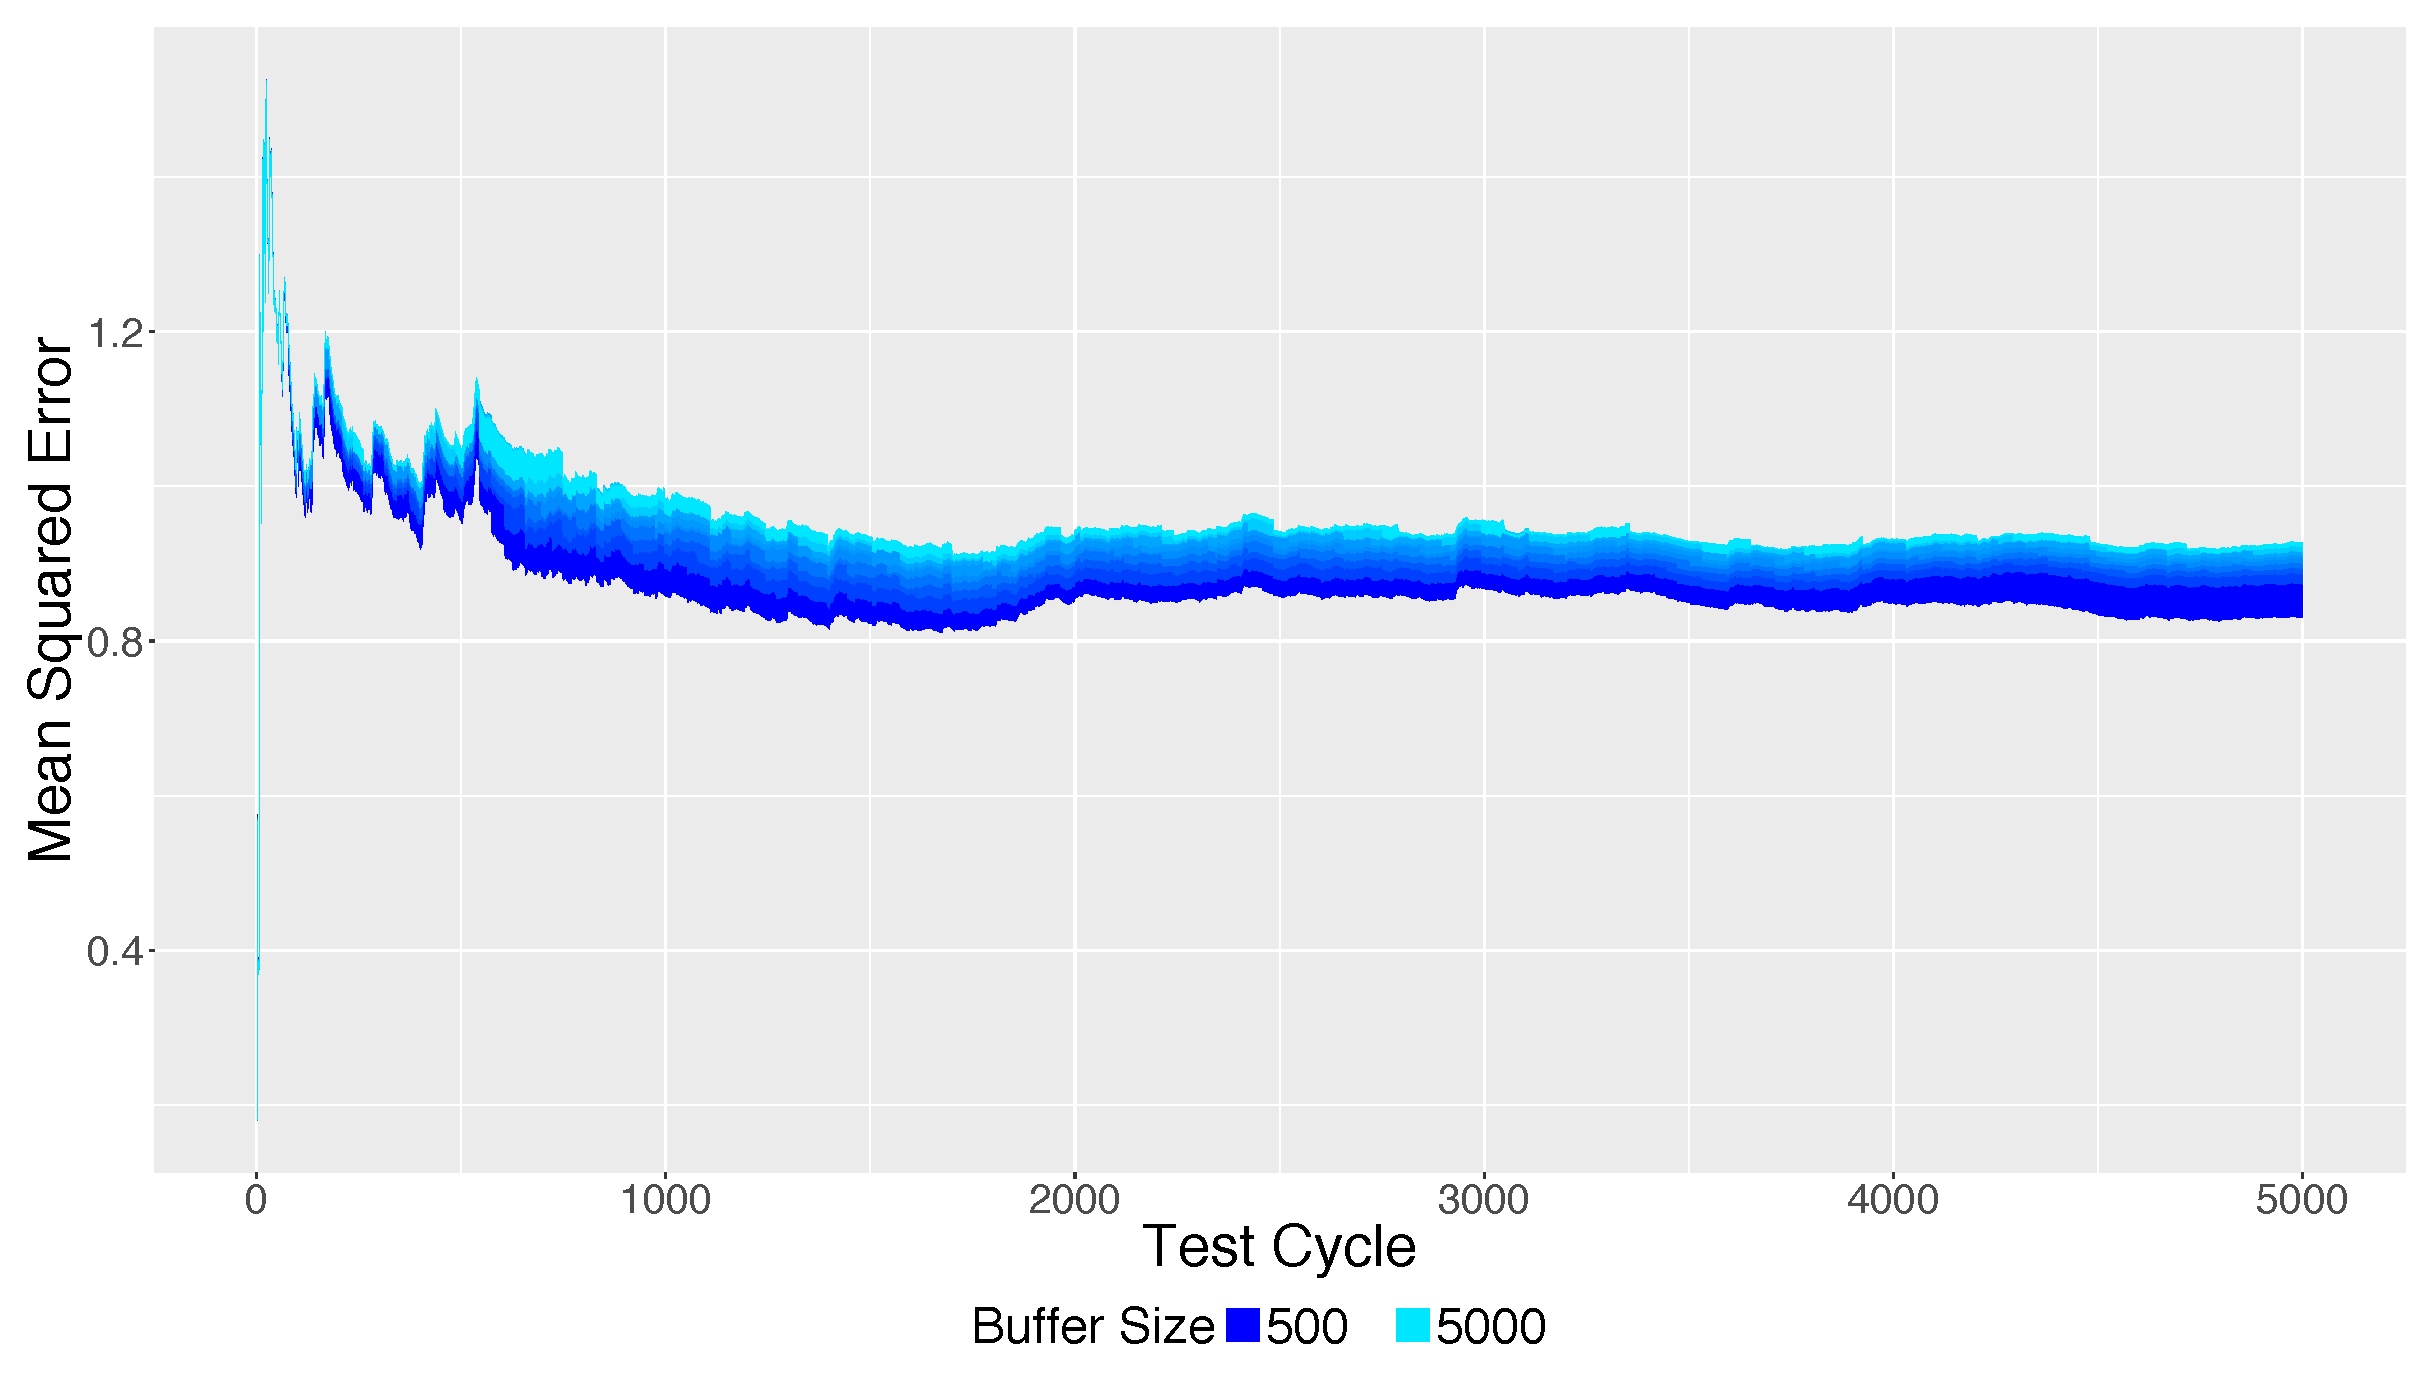
\includegraphics[width=\columnwidth]{../images/experiment-results/movie-lens-100k-buffer-size-improved.eps}
\caption{Movie Lens 100k buffer size vs mean squared error}
\label{fig:movie-lens-100k-buffer-size-mse}
\end{figure}

Figure \ref{fig:movie-lens-100k-buffer-size-mse} shows the mean squared error for different buffer sizes for \textit{movie-lens-100k} dataset. 
An smaller buffer size causes the scheduler to initiate training iterations more frequently.
As a result, the underlying model is updated faster.
However, the error rate is not decreasing linearly with the buffer size.
Further analysis show that once the model is update more frequently, it slowly starts to converge and any further training has little to no effect on the overall quality of the model
Therefore, increasing the scheduling rate only decreases the error rate up to a point, after which increasing the scheduling rate has no effect on the overall quality of the model.
This is extremely important, specially when considering the effect the buffer size has on the running time.
Figure \ref{fig:movie-lens-100k-buffer-size-time} shows the running time on \textit{movie-lens-100k} dataset using different buffer sizes. 
Increasing the buffer size from 500 to 5000 decreases the running time by a factor of 5 while as described before the error rate is only increased slightly.
Therefore, depending on the application, we can set the buffer size to bigger values in order to increase the performance of the system without affecting the quality of the final model substantially.

\begin{figure}[H]
\centering
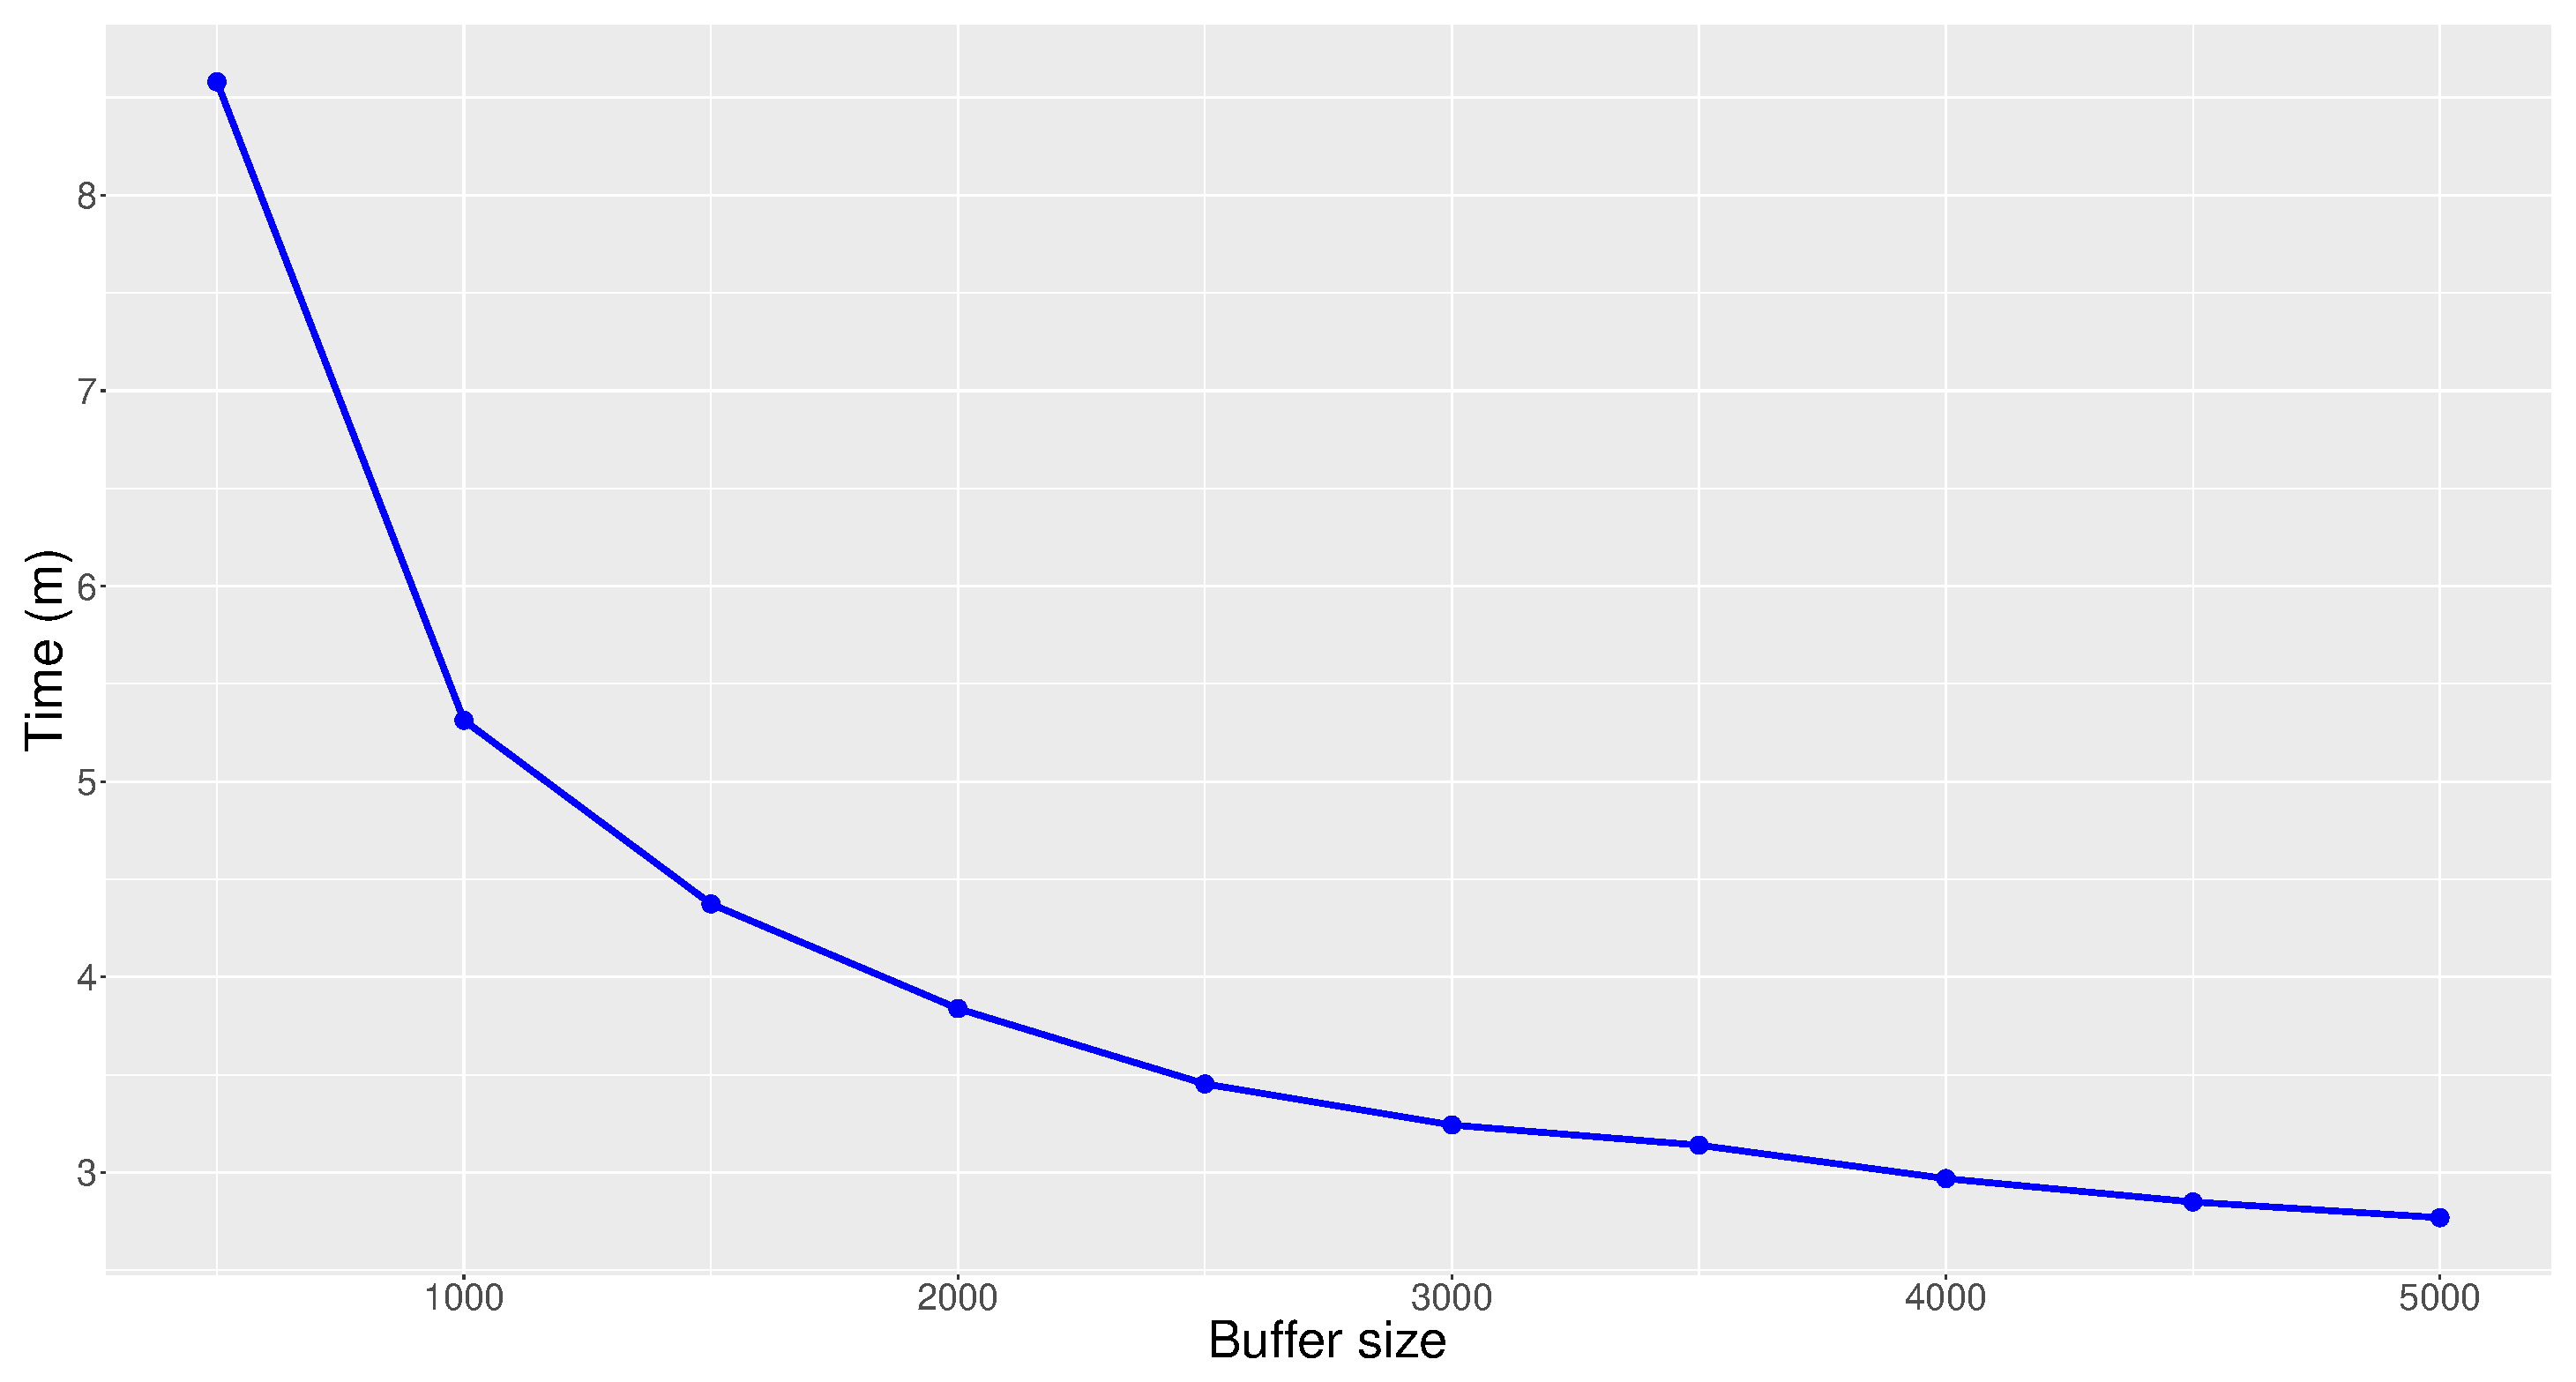
\includegraphics[width=\columnwidth]{../images/experiment-results/movie-lens-100k-buffer-time-improved.eps}
\caption{Movie Lens 100k buffer size vs time}
\label{fig:movie-lens-100k-buffer-size-time}
\end{figure}

\textit{Dynamic scheduling:} In production environments, the load on the system varies throughout the day. 
Therefore, a dynamic scheduling maximizes the performance of the system, by performing more frequent updates while there are more resources available for training. 
Moreover, since training and serving can be done in parallel, we can perform training in the background and only update the weights when the training iteration is over. 

\textbf{Sampling rate:} In each iteration of SGD, as described in Section \ref{continious-training-serving}, the data inside the buffer and a sample of the historical data is used to update the model.
In this section, we investigate the effect of the sampling rate on the model quality and running time of the system.
Figure \ref{fig:movie-lens-100k-sample-rate} shows that larger sampling rate increases the quality of the model, but similar to scheduling rate, the decrease in error rate is negligible considering the effect it has on running time. 
This is again, caused by the same phenomena, where the model after training on bigger sample rates start to converge faster and as a result bigger sample sizes will not have an effect on the quality.
 
\begin{figure}[!ht]
\centering
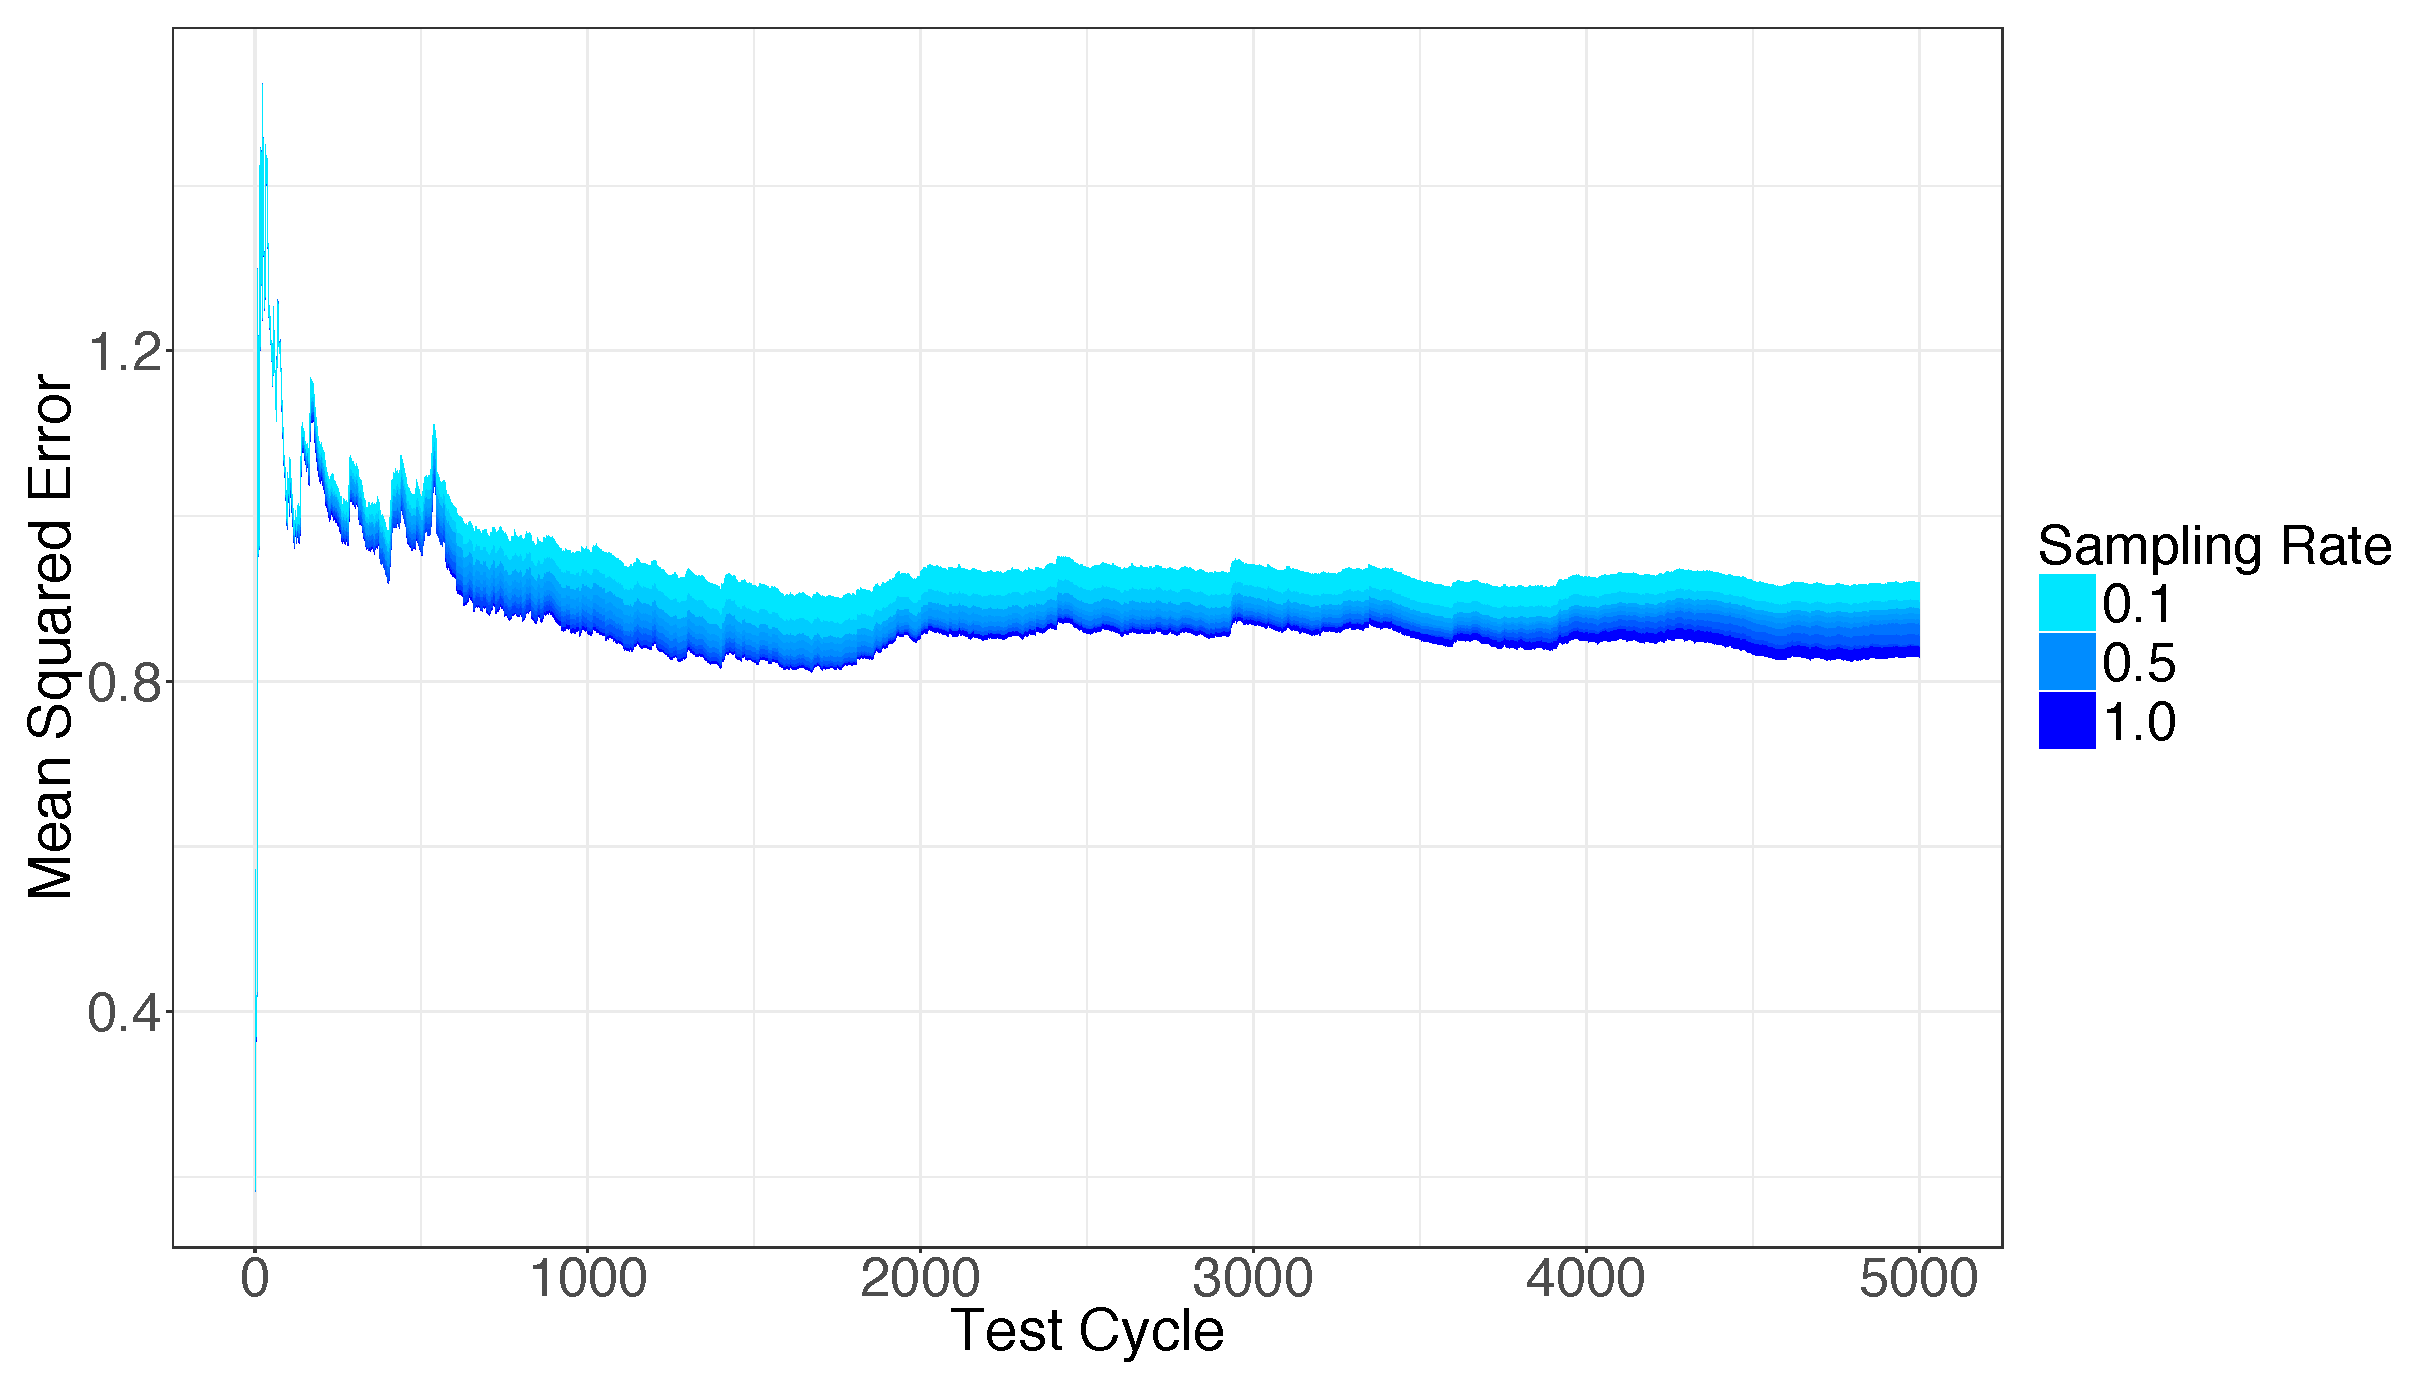
\includegraphics[width=\columnwidth]{../images/experiment-results/movie-lens-100k-sampling-rate-improved.eps}
\caption{Movie Lens 100k sample rate vs mean squared error}
\label{fig:movie-lens-100k-sample-rate}
\end{figure}

Figure \ref{fig:movie-lens-100k-sample-rate-time} shows that effect of increasing sampling rate on running time.
Using the entire historical data (sampling rate = 1.0) increases the running time 5 fold. 
Therefore, similar to scheduling rate, setting the sampling rate to smaller values will increase the performance substantially, while only slightly affecting the quality of the model.


\begin{figure}[H]
\centering
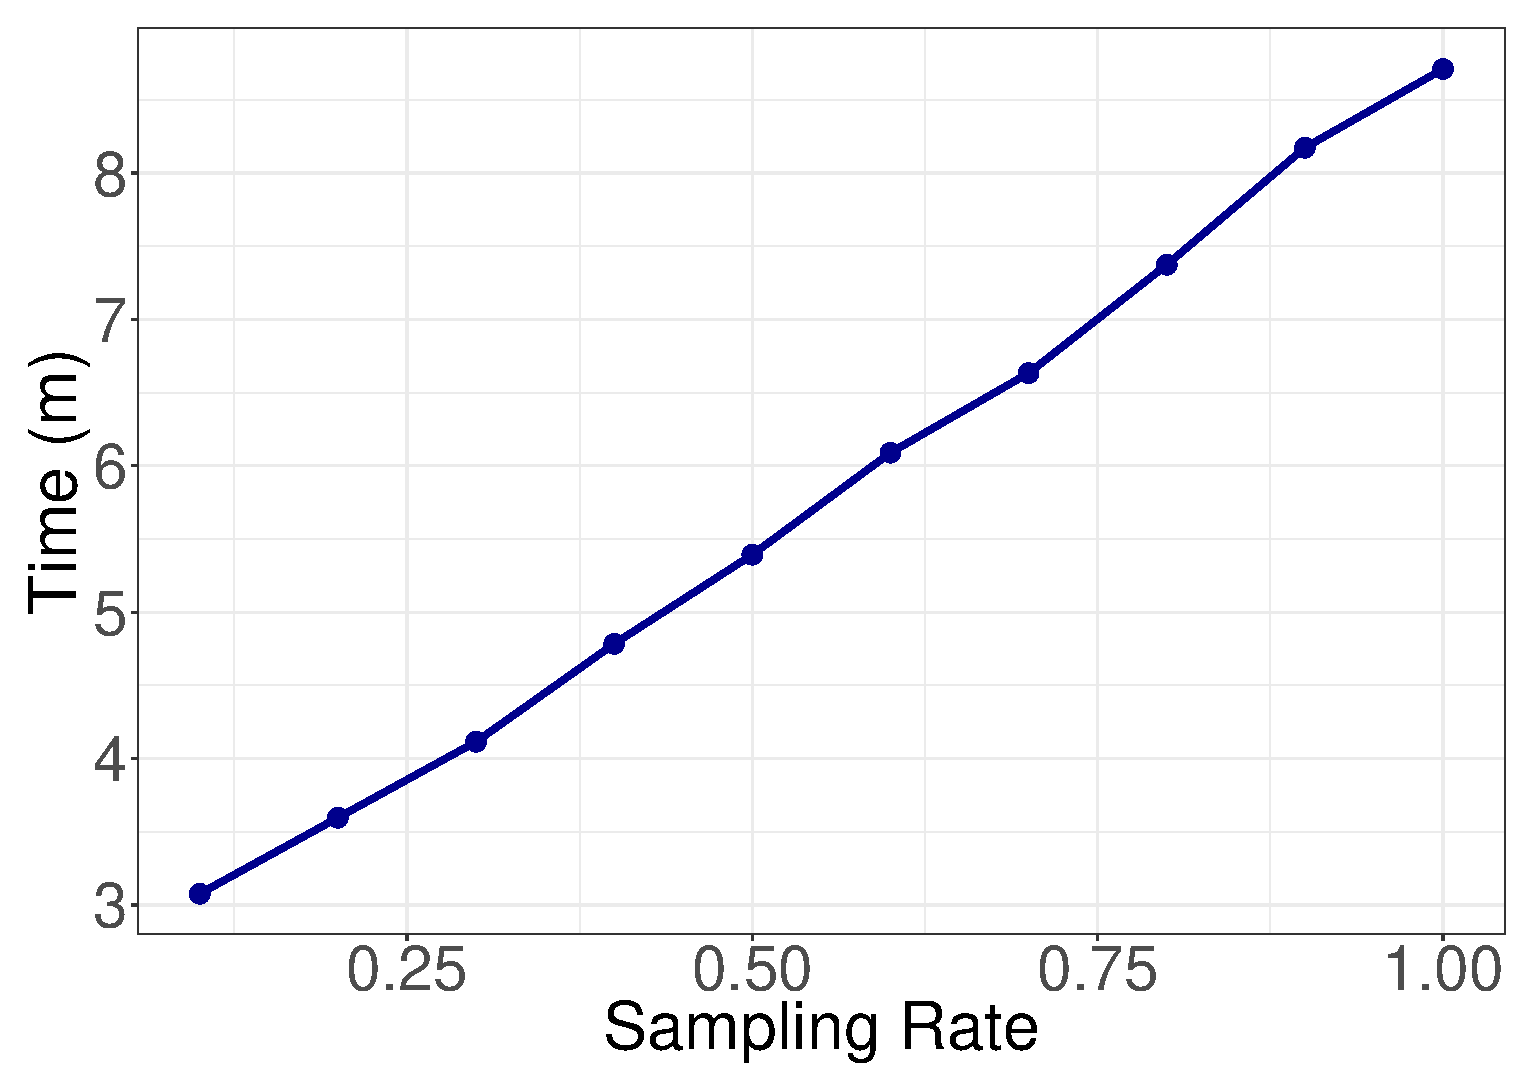
\includegraphics[width=\columnwidth]{../images/experiment-results/movie-lens-100k-sampling-time-improved.eps}
\caption{Movie Lens 100k sampling rate vs time}
\label{fig:movie-lens-100k-sample-rate-time}
\end{figure}

\textbf{Tuning parameters based on error rate:} As described earlier, tuning the parameters are heavily influenced by application type.
Both the underlying machine learning model and the dataset can have a big effect on the selection of sampling rate and scheduling rate.
In the recommender system use case, due to changes in incoming data distribution, we saw that bigger sample rates and higher scheduling rates have an effect (although small) on the quality of the model.
This, however, may not be the case for other use cases.
To demonstrate this, we perform the same set of experiments on the \textit{MNIST} dataset.
Figure \ref{fig:mnist-sample-rate} shows the effect of different sampling rates on the neural network model for \textit{MNIST} data.
Interestingly and contrary to the results we achieved for \textit{movie-lens-100k} the difference in error rates for different sampling rates are almost indistinguishable from each other.
While the difference in error rates for \textit{movie-lens-100k} was small, but it is still much greater than the difference in error rates for neural networks.
We believe this is caused by how neural networks behave.
Increasing sampling rate, causes similar data items to be used repeatedly in each training iteration and based on our experiments neural networks are not affected by this oversampling and, therefore, the results are almost similar with different sampling rates.
Moreover, in this experiment, the number of parameters of multi-layer perceptron is far less than the number of parameters of the matrix factorization model for \textit{movie-lens-100k}.
This causes the neural work to converge faster and, therefore, it is not affected by more training, unless new training observations arrive at the system.

\begin{figure}[!ht]
\centering
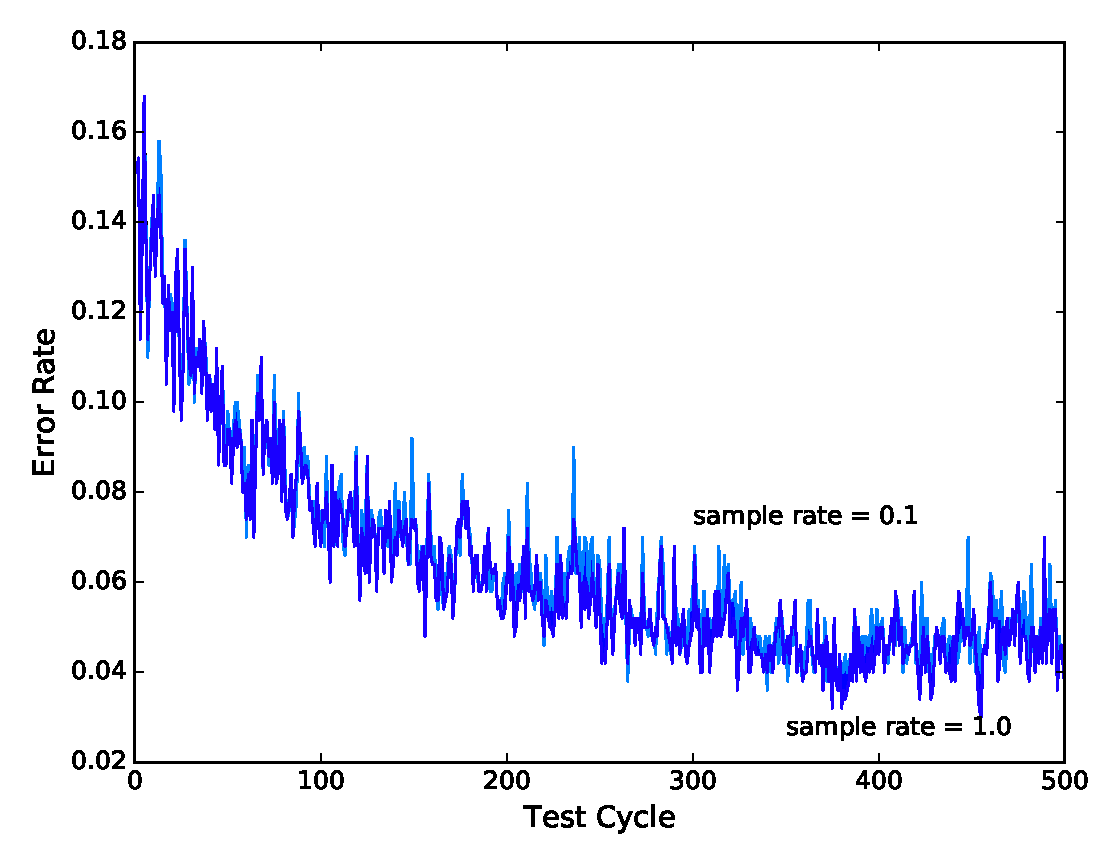
\includegraphics[width=\columnwidth]{../images/experiment-results/mnist-sampling.eps}
\caption{MNIST sample rate vs error rate}
\label{fig:mnist-sample-rate}
\end{figure}

Figure \ref{fig:mnist-buffer-size} shows how buffer size affects the overall quality of the neural network models achieved.
Similar to sampling rate case, the error rates of the models are not affected by the scheduling rate.
New training observations that exist in the buffer have the maximum effect on the model's quality, since they are becoming available to the model for the first time.
As the scheduling rate increases, the number of new training observations remain the same, and only the historical data is used more frequently to train the model.
Since neural networks do not gain much benefit by revisiting the same items, increasing scheduling rate has no effect on the overall quality.

Based on our findings, we conclude that increasing the sampling and scheduling rate does not always have an effect on the quality.
In both the \textit{movie-lens-100k} and \textit{MNIST} use cases the change in scheduling and sampling rate has small to no effect on the overall quality.
However, the running time of the methods are heavily influenced by these parameters.
Setting these parameters to small values decreases the running time considerably and save computation resources regardless of the type of model the system is serving.


\begin{figure}[!ht]
\centering
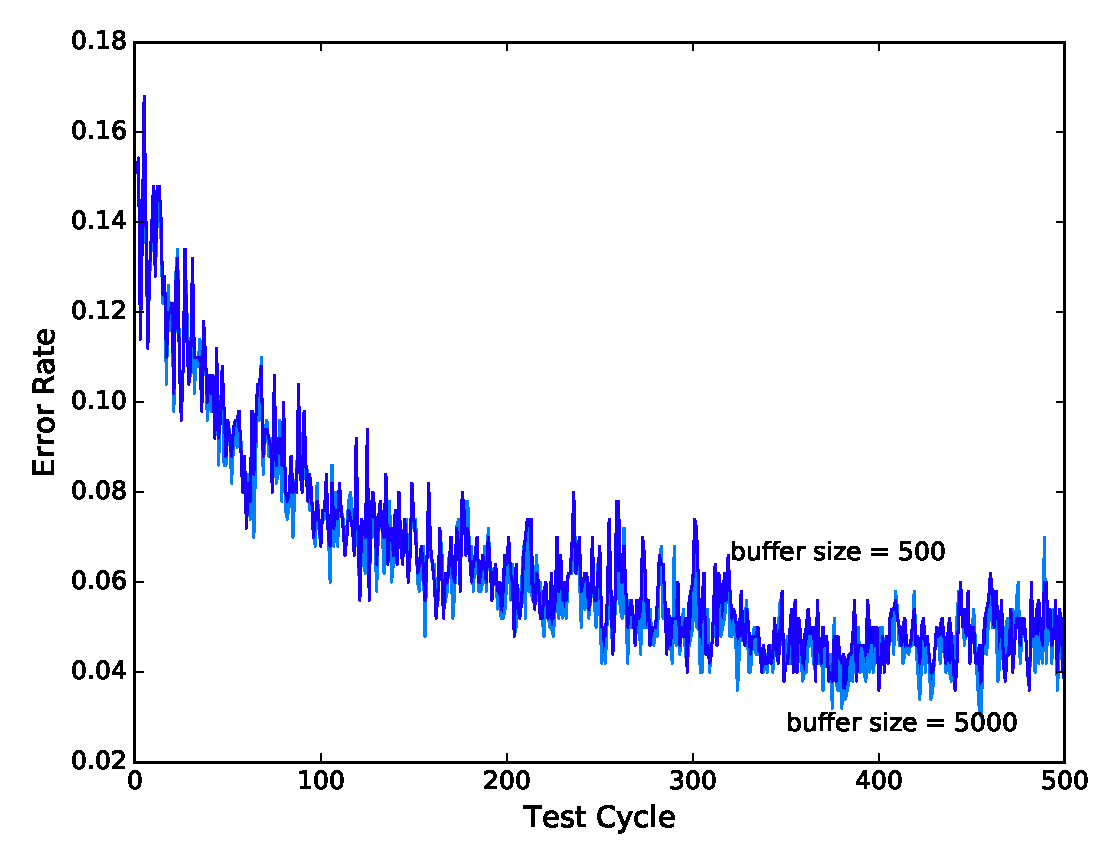
\includegraphics[width=\columnwidth]{../images/experiment-results/mnist-buffer-size}
\caption{MNIST buffer size vs error rate}
\label{fig:mnist-buffer-size}
\end{figure}



\subsection{Comparison Under Constrained Resources }
Both, the velox and the continuous model use different strategies to update the model.
To perform a fair comparison of the two, we are evaluating them under similar resource constraints.
We configured both of the methods' frequency of training in such a way that the total running time on the \textit{movie-lens} and \textit{MNIST} datasets are similar.
To achieve this, we have fixed the total number of epochs (SGD iterations) for both methods.
For velox, this value is equal to the number of retraining multiplied by number of iterations in each retraining. 
For the continuous model, it is total number of scheduled iterations throughout the lifetime of the system.
Therefore, the continuous method schedules a new iteration every 500 items for \textit{movie-lens-100k} and 5,000 items for \textit{movie-lens-1M} and velox method schedules a retraining every 15,000 items for \textit{movie-lens-100k} and 150,000 items for \textit{movie-lens-1M}.
\begin{figure}[h]
\centering
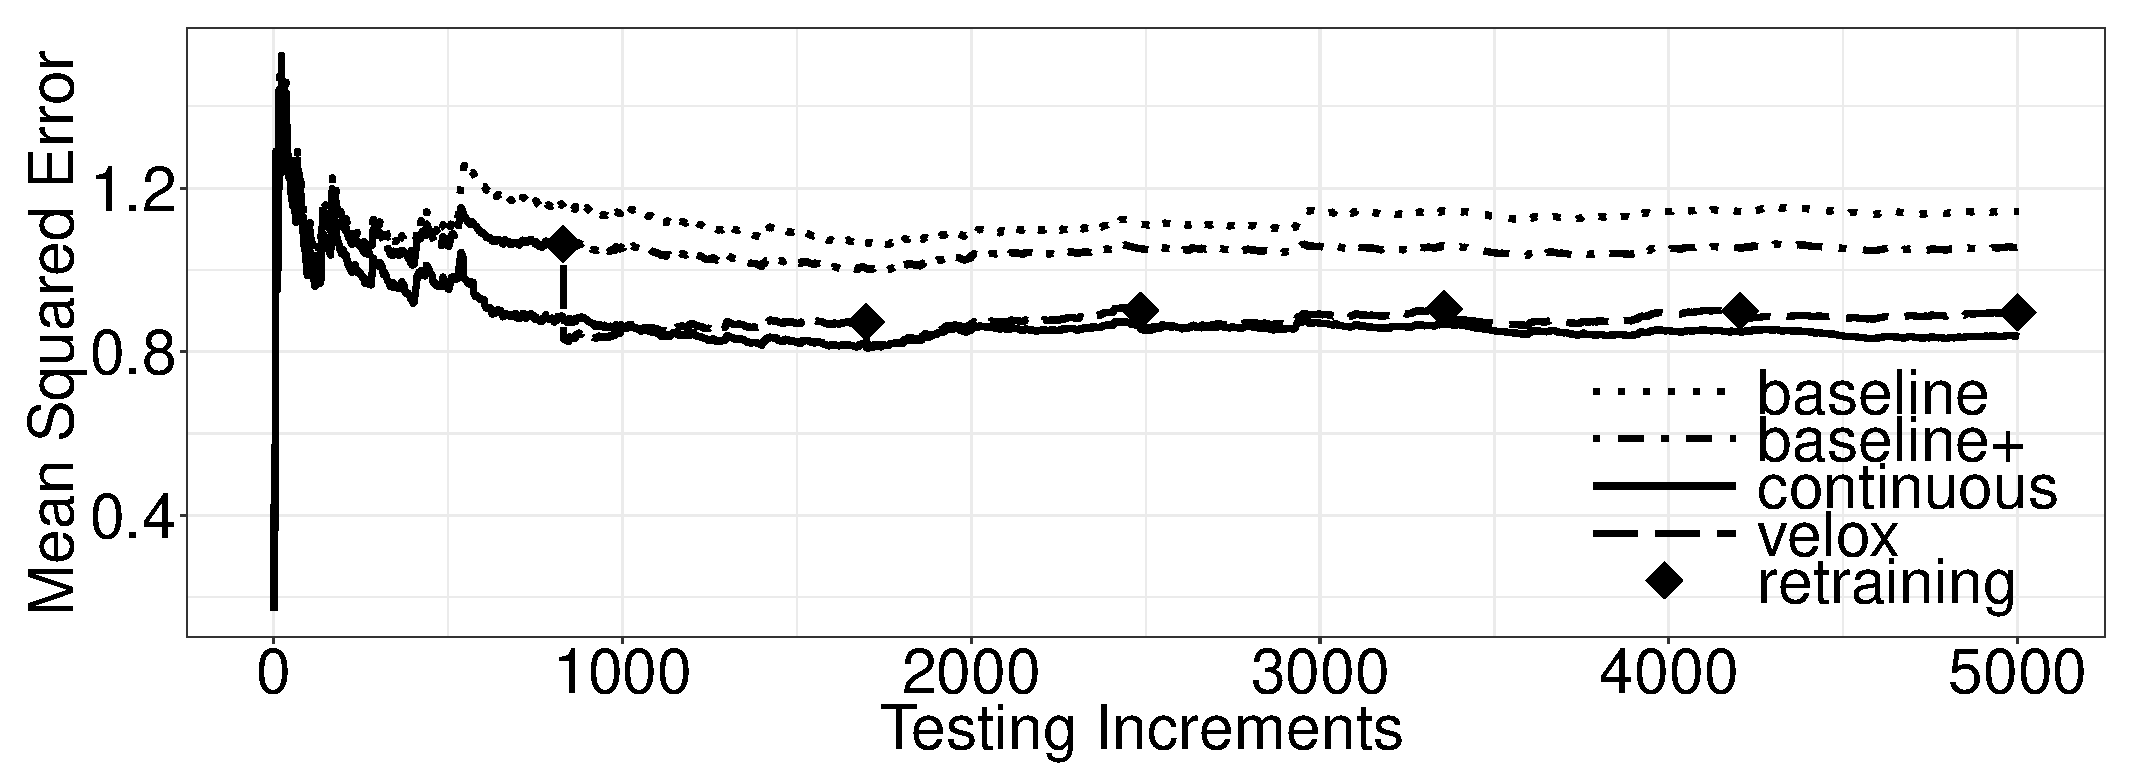
\includegraphics[width=\columnwidth]{../images/experiment-results/movie-lens-100k-quality-improved.eps}
\caption{Mean squared error on MovieLens 100k}
\label{fig:movie-lens-100k-score}
\end{figure}
Figure \ref{fig:movie-lens-100k-score} shows the mean squared error of the continuous, velox, and several other methods on \textit{movie-lens-100k} dataset.
Baseline model achieves the worst performance among all the existing methods.
Baseline model's quality is similar to Baseline+, Continuous, and Velox methods in the beginning. 
Since all four methods perform an initial retraining, the error rate stays low in the beginning, but Baseline quality starts to degrade since it does not include any incremental or batch retraining.
Baseline+ continuous to perform better than naive method until 3,000 test cycles.
However, afterwards a small change in distribution of the data causes the model trained using Baseline method to perform worst since it cannot adopt to changes in the data and the quality continues to degrade as more new test items are examined.
Velox method performs similar to Baseline+ method until the first retraining is executed.
There is a sudden drop in the error rate after the first retraining.
For the remainder of the data points, Velox performs as expected, once there is a retraining, the error rate immediately decreases.
This decrease in error rate, however, is followed by a slow increase due the fact that only incremental updates are being made to the model.
Finally, Continuous method has the lowest error rate among all the implemented methods.
It consistently manages to adopt to the changes and decrease the error rate where the distribution of the incoming data is stable.
As expected, except for immediately after a full retraining, the Continuous method always performs better than Velox.

\begin{figure}[h]
\centering
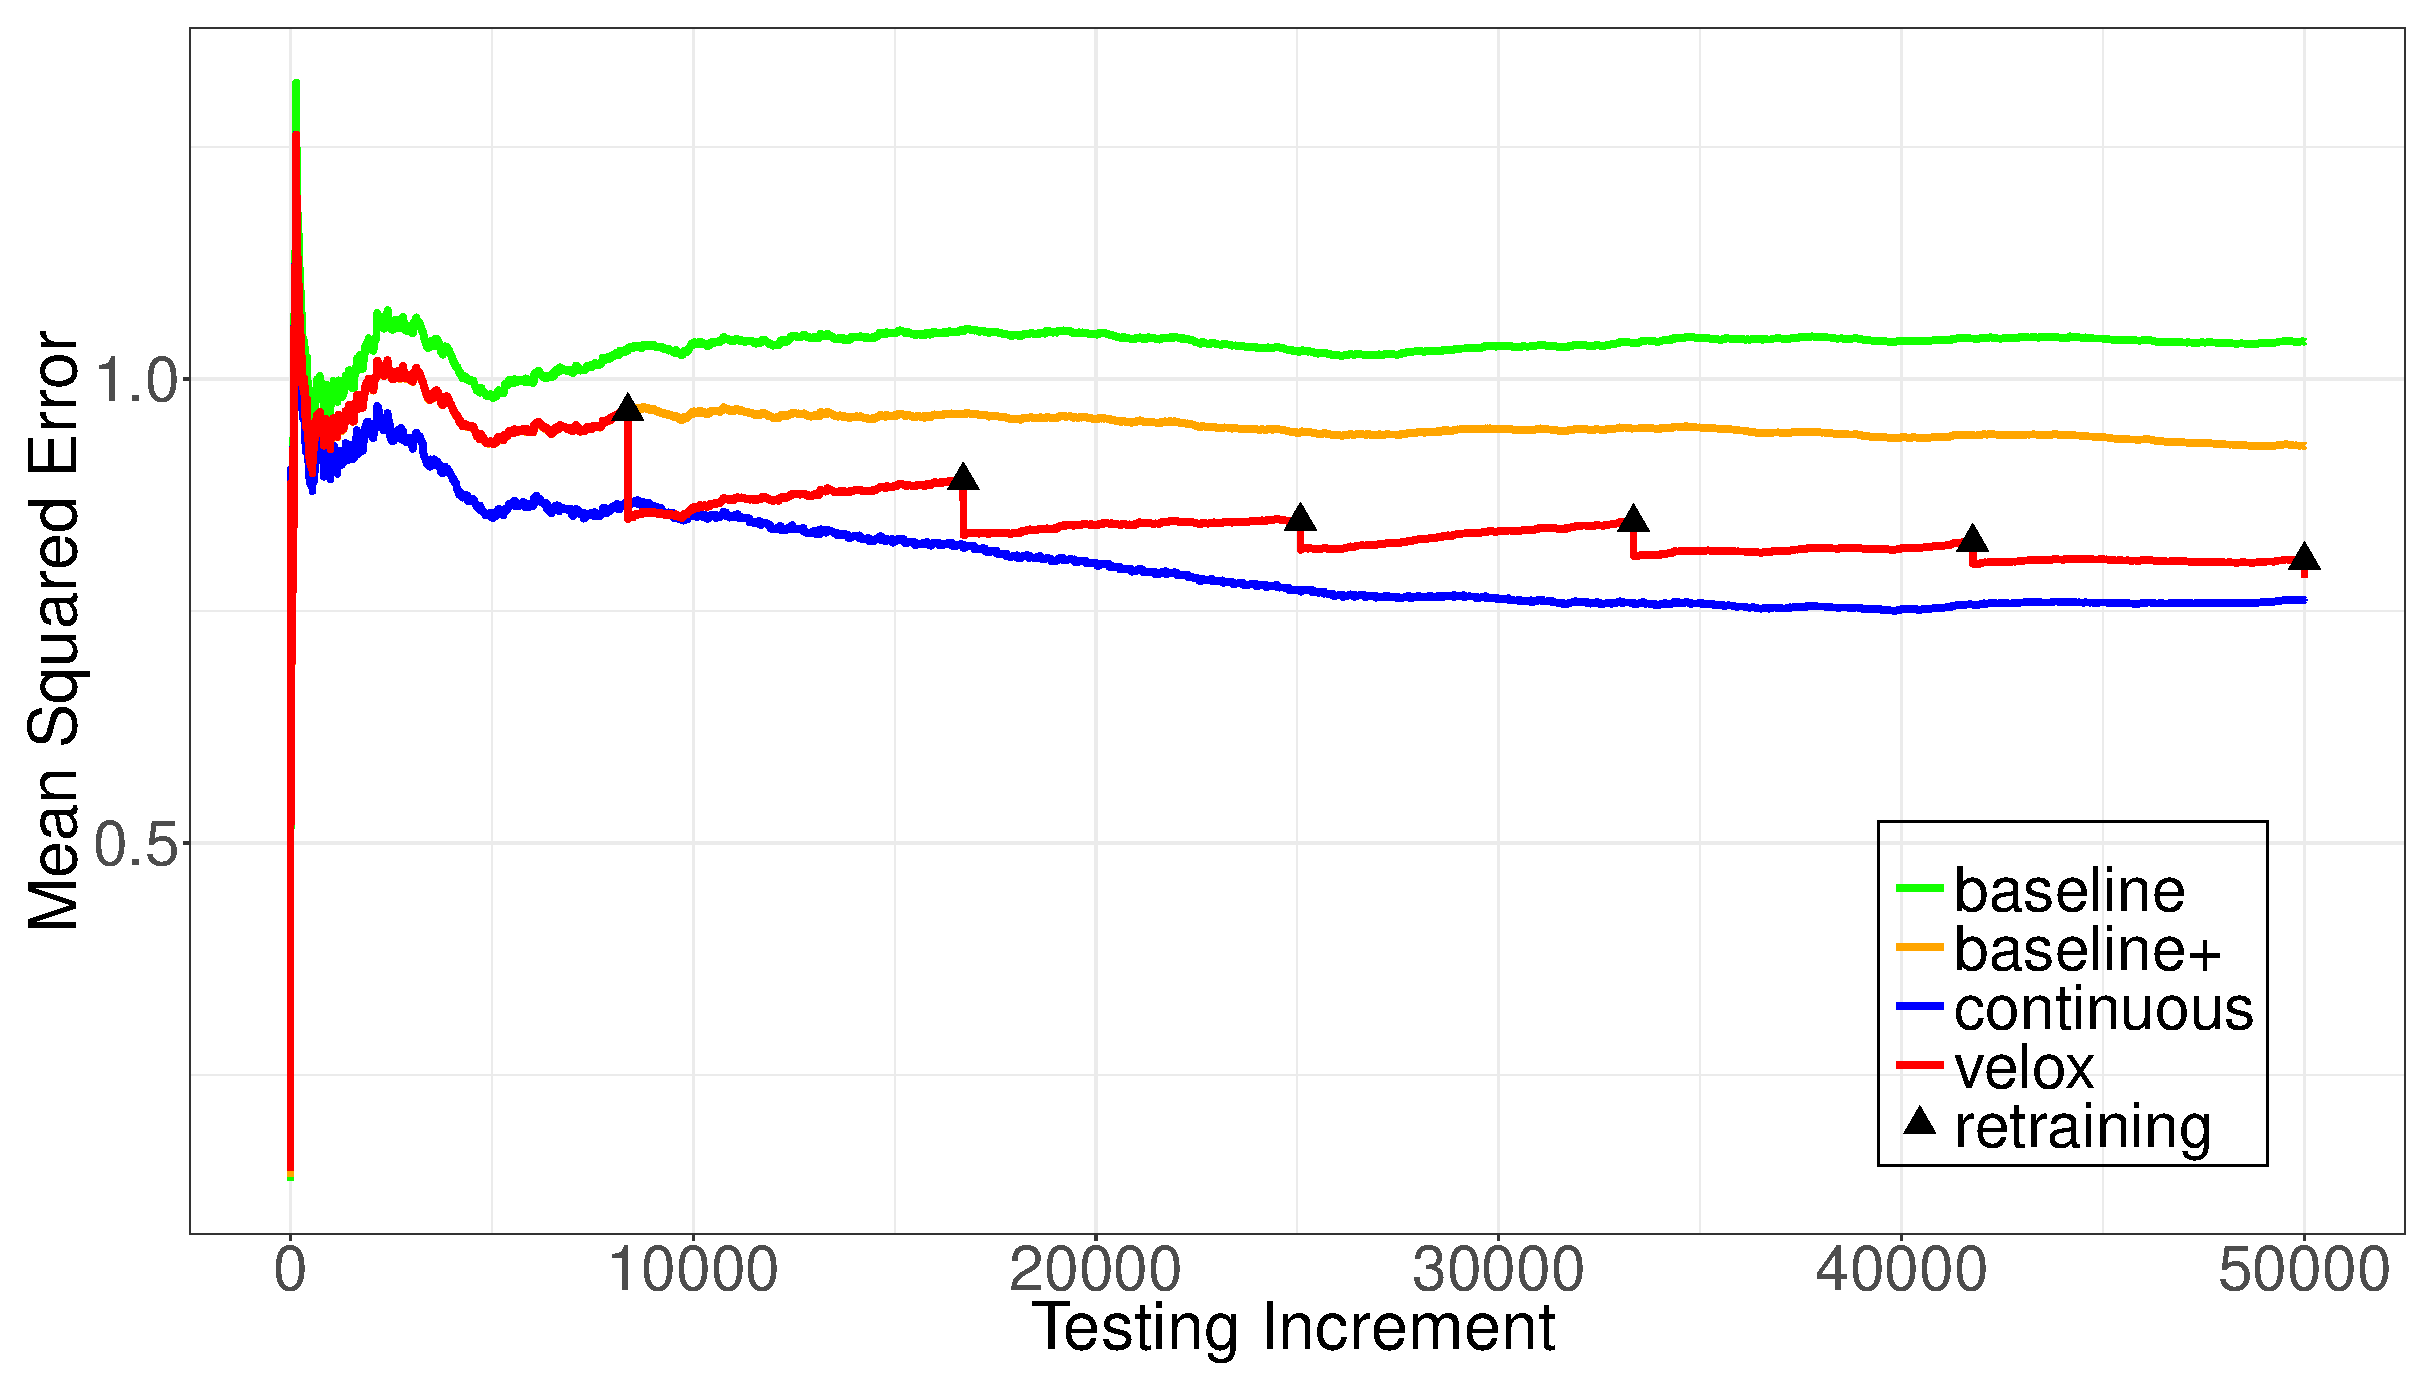
\includegraphics[width=\columnwidth]{../images/experiment-results/movie-lens-1m-quality-improved.eps}
\caption{Mean squared error on Movie Lens 1M}
\label{fig:movie-lens-1M-score}
\end{figure}

Figure \ref{fig:movie-lens-1M-score} shows the mean squared error rate achieved by the implemented methods on \textit{movie-lens-1M}.
Similar to \textit{movie-lens-100k}, the Continuous method has the lowest error rate among all the implemented methods.
The difference in error rate between Continuous and Velox is even greater than the error rate for \textit{movie-lens-100k}.
We believe a bigger shift in data distribution (data in \textit{movie-lens-1M} is gathered from a longer period of time) makes the Continuous method to consistently adopt faster to the changes in data distribution.
Velox's error rate follows the same trend as in the case of \textit{movie-lens-100k}. 
After every retraining, the error rate first drops then slowly increases until the next retraining.
Similar to \textit{movie-lens-100k} dataset, the error rate of Baseline is highest among all the implemented methods, followed by Baseline+ , where due to the incremental updates of the model the error rate is consistently lower.




\begin{figure}[h]
 \centering
 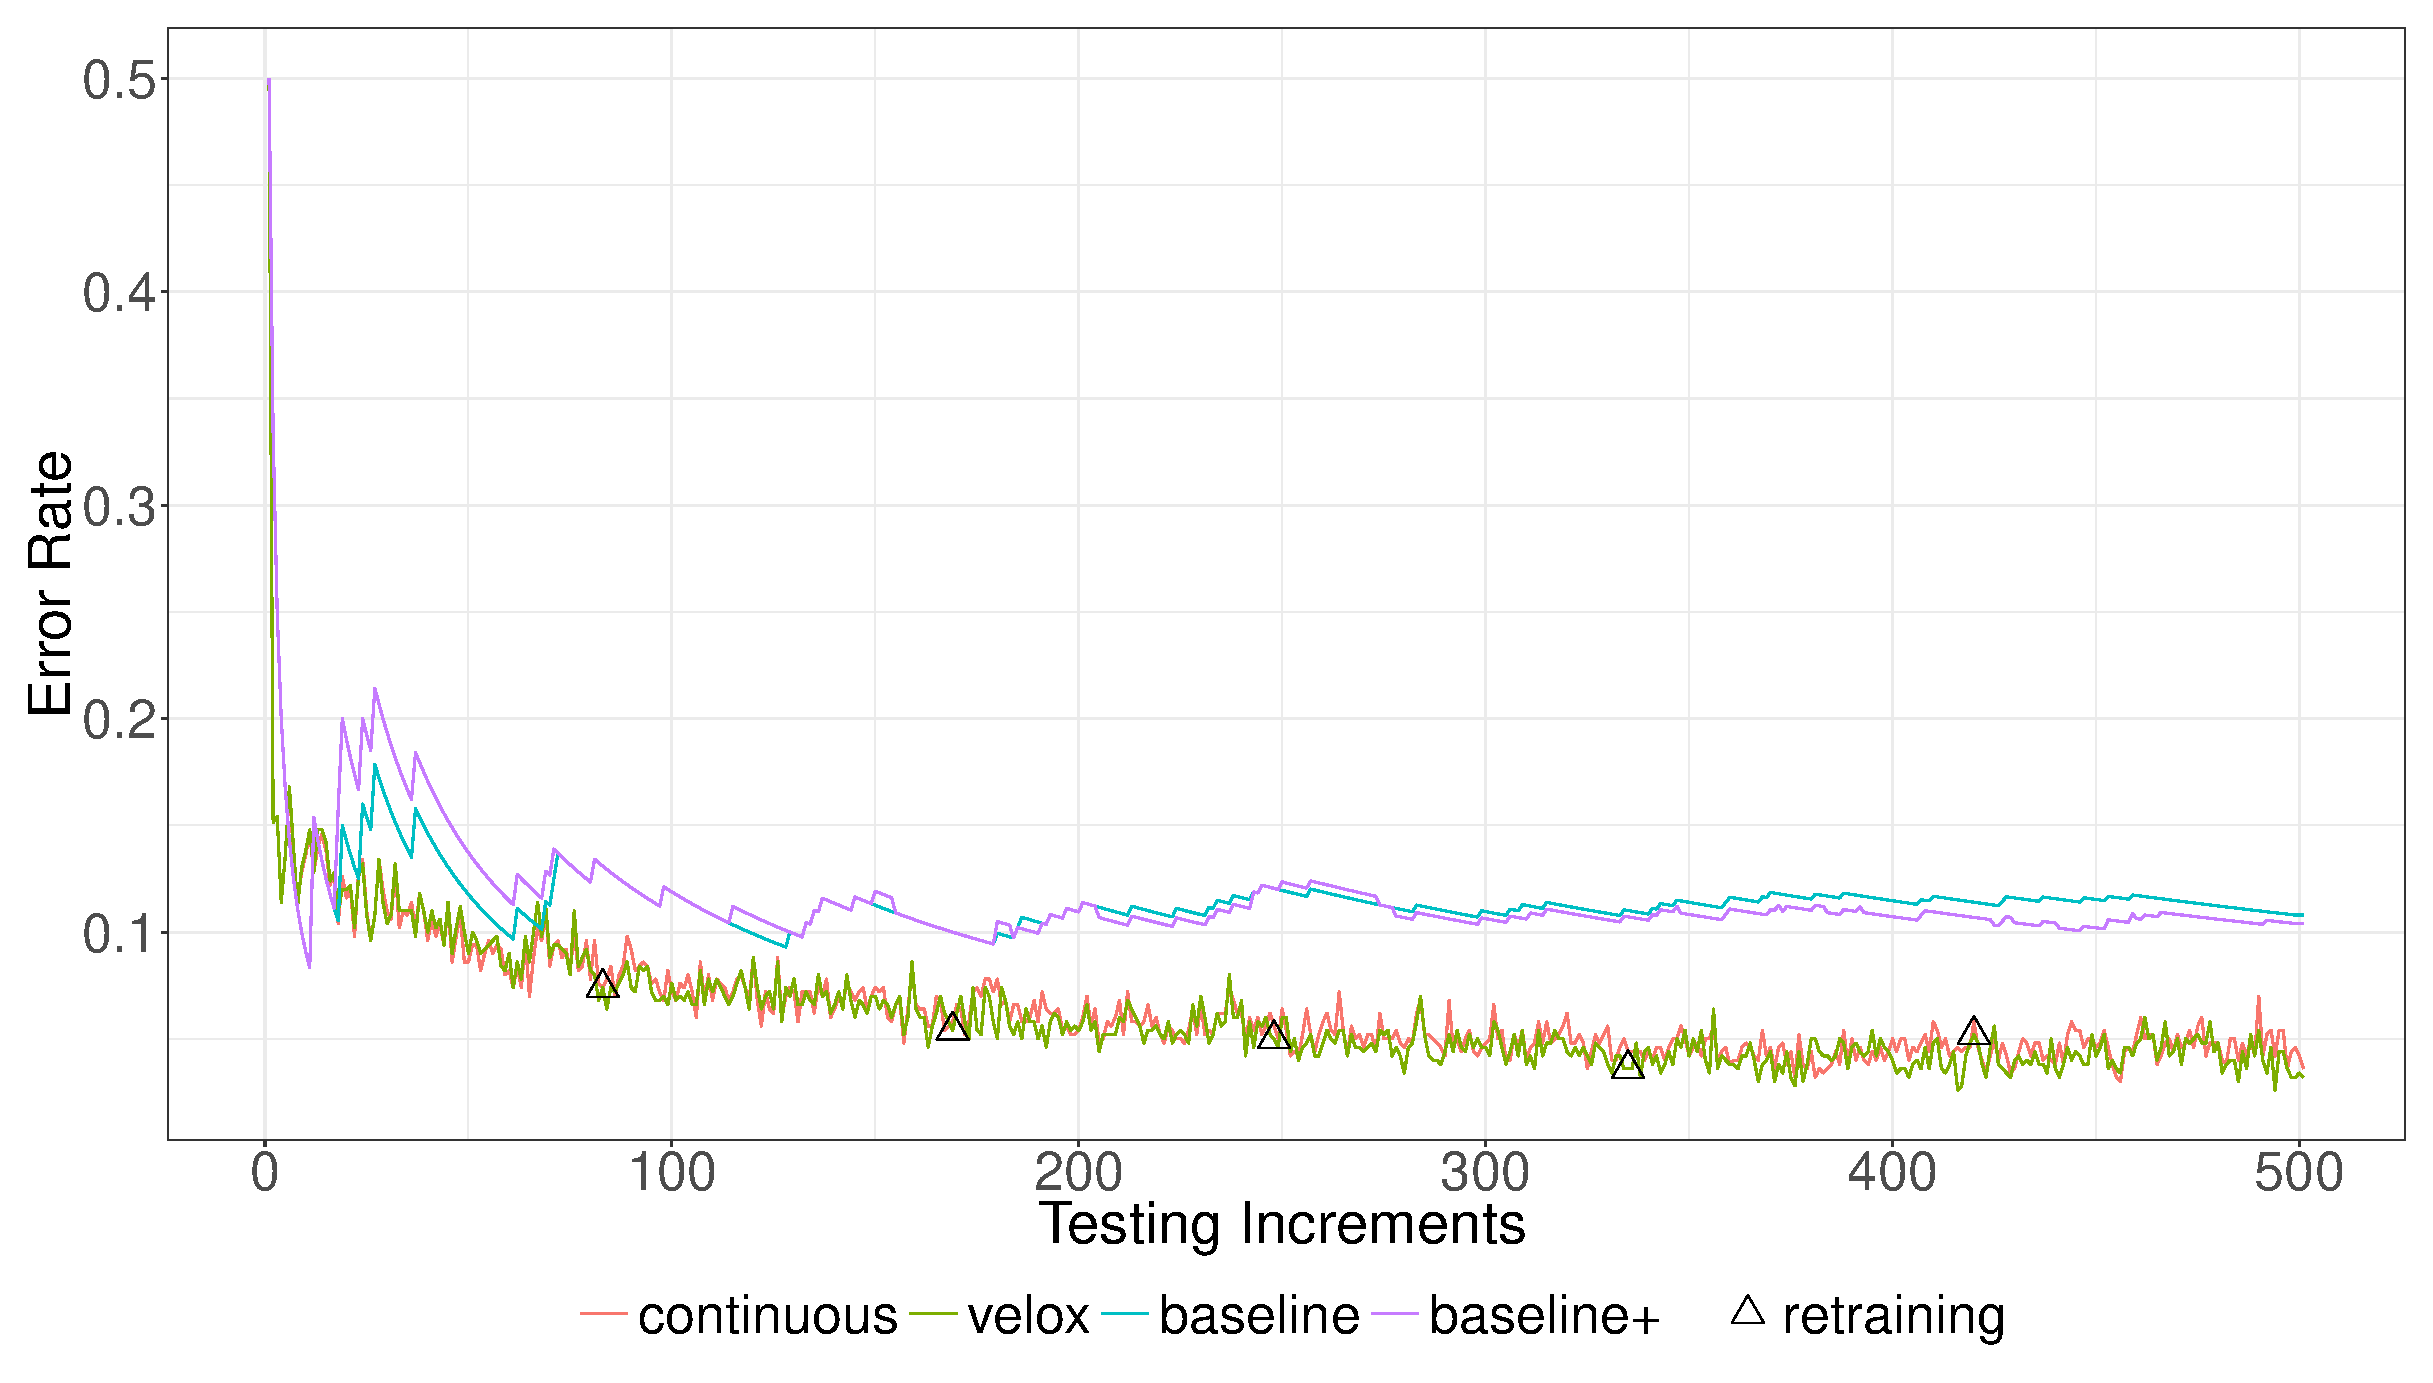
\includegraphics[width=\columnwidth]{../images/experiment-results/mnist-quality.eps}
 \caption{Error rate on MNIST}
 \label{fig:mnist-quality}
 \end{figure}
 
Figure \ref{fig:mnist-quality} shows the error rate (misclassification rate) of the implemented methods on \textit{MNIST} dataset.
For this workload, the implemented methods behave quite differently from previous experiments and that is due to dataset characteristics and the underling model properties.
In order to achieve a high accuracy, neural networks require a lot of training data.
This explains why the naive method performs poorly.
Its error rate starts to decrease as more training data becomes available, but it is still far inferior to all the other methods.
The gap in error rate between offline+online and offline-only methods is much smaller than that of movie lens datasets.
Unlike the movie lens datasets, \textit{MNIST} does not contain a shift in distribution and that is why both the offline+online and offline-only methods' performance is rather similar.
The Baseline+ method performs slightly better because of the extra training items that the underlying neural network is exposed to.
Velox and Continuous methods behave similarly as well and unlike Movie Lens datasets, Velox has a consistent error rate, that is the error rate does not decrease after a retraining of the model.
Similar to offline+online's case, since there is no change in the distribution of the data, the error rate does not degrade after a retraining.
The continuous method manages to decrease the error rate as more training iterations are performed.
As more training iterations are executed, the underlying neural network's parameters converge and as a result the error rate on the test set decreases.
Both Continuous and Velox start to perform better than the baseline after a few training iterations (retraining in Velox's case).
This is, as explained earlier because of neural network's ability to perform better when more training data are available to it.

\begin{figure}[h]
\centering
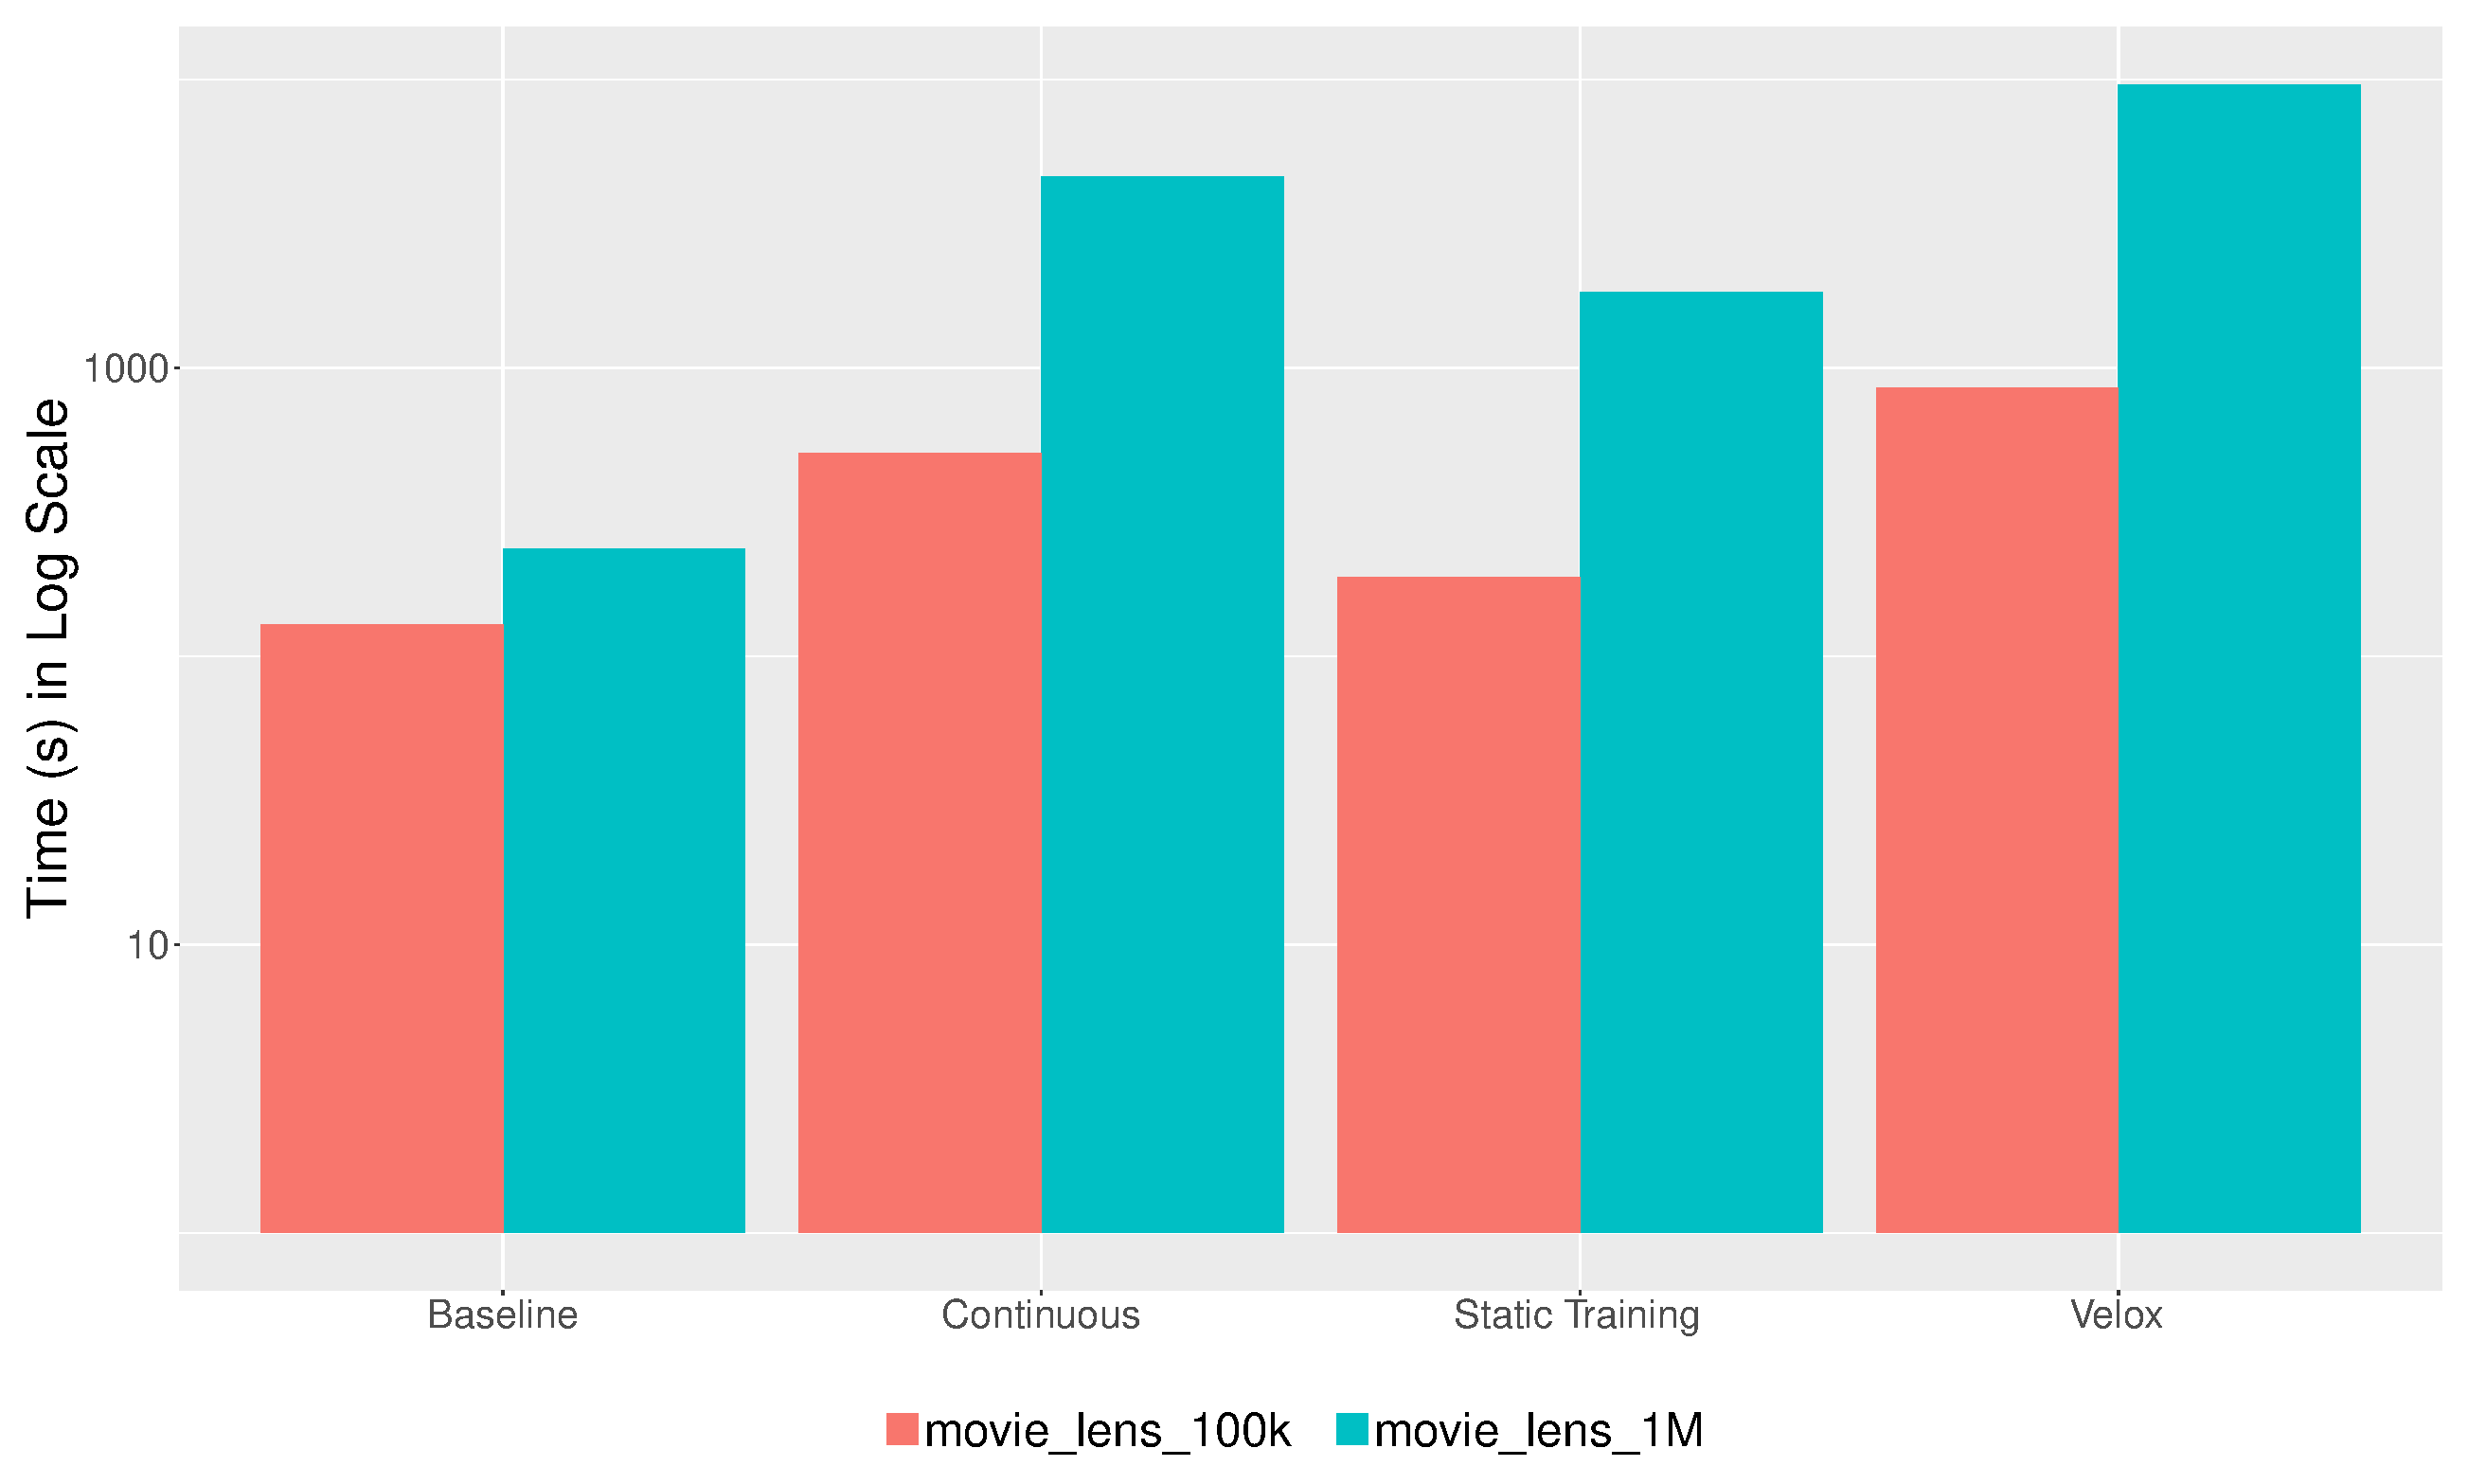
\includegraphics[width=\columnwidth]{../images/experiment-results/times-log-scale-improved.eps}
 \caption{Running time on different Workloads}
 \label{fig:running-time}
 \end{figure}
Figure \ref{fig:running-time} shows the running time of the implemented methods on \textit{movie-lens-100k}, \textit{movie-lens-1M} and \textit{MNIST}.
As expected, Baseline have the lowest running times on both datasets.
This is because they do not support batch updates to the model.
Static training method's running time is only affected by data size.
When dataset size big, each iteration of SGD will examine more data and the model will converge slower as there are a lot more data to examine.
Continuous method's running time is smaller than Velox by almost an order of magnitude in all workloads.
Although we have configured both methods to use similar amount of resources (same number of iterations), continuous method still manages to achieve a consistent and lower error rate in a much faster time.
This is because a full retraining incurs a much higher overhead than continuously training the method.
Another reason for the difference in running time is that as the size of the data increases the time for running a new iteration in continuous method stays roughly the same where as the time for a full retraining increases exponentially.
The running time of the Baseline+ is not included as it is similar to Baseline, since they both have include initial training and have to examine individual items arriving at the system one at a time.

\begin{figure*}[h]
\begin{subfigure}{.5\textwidth}
  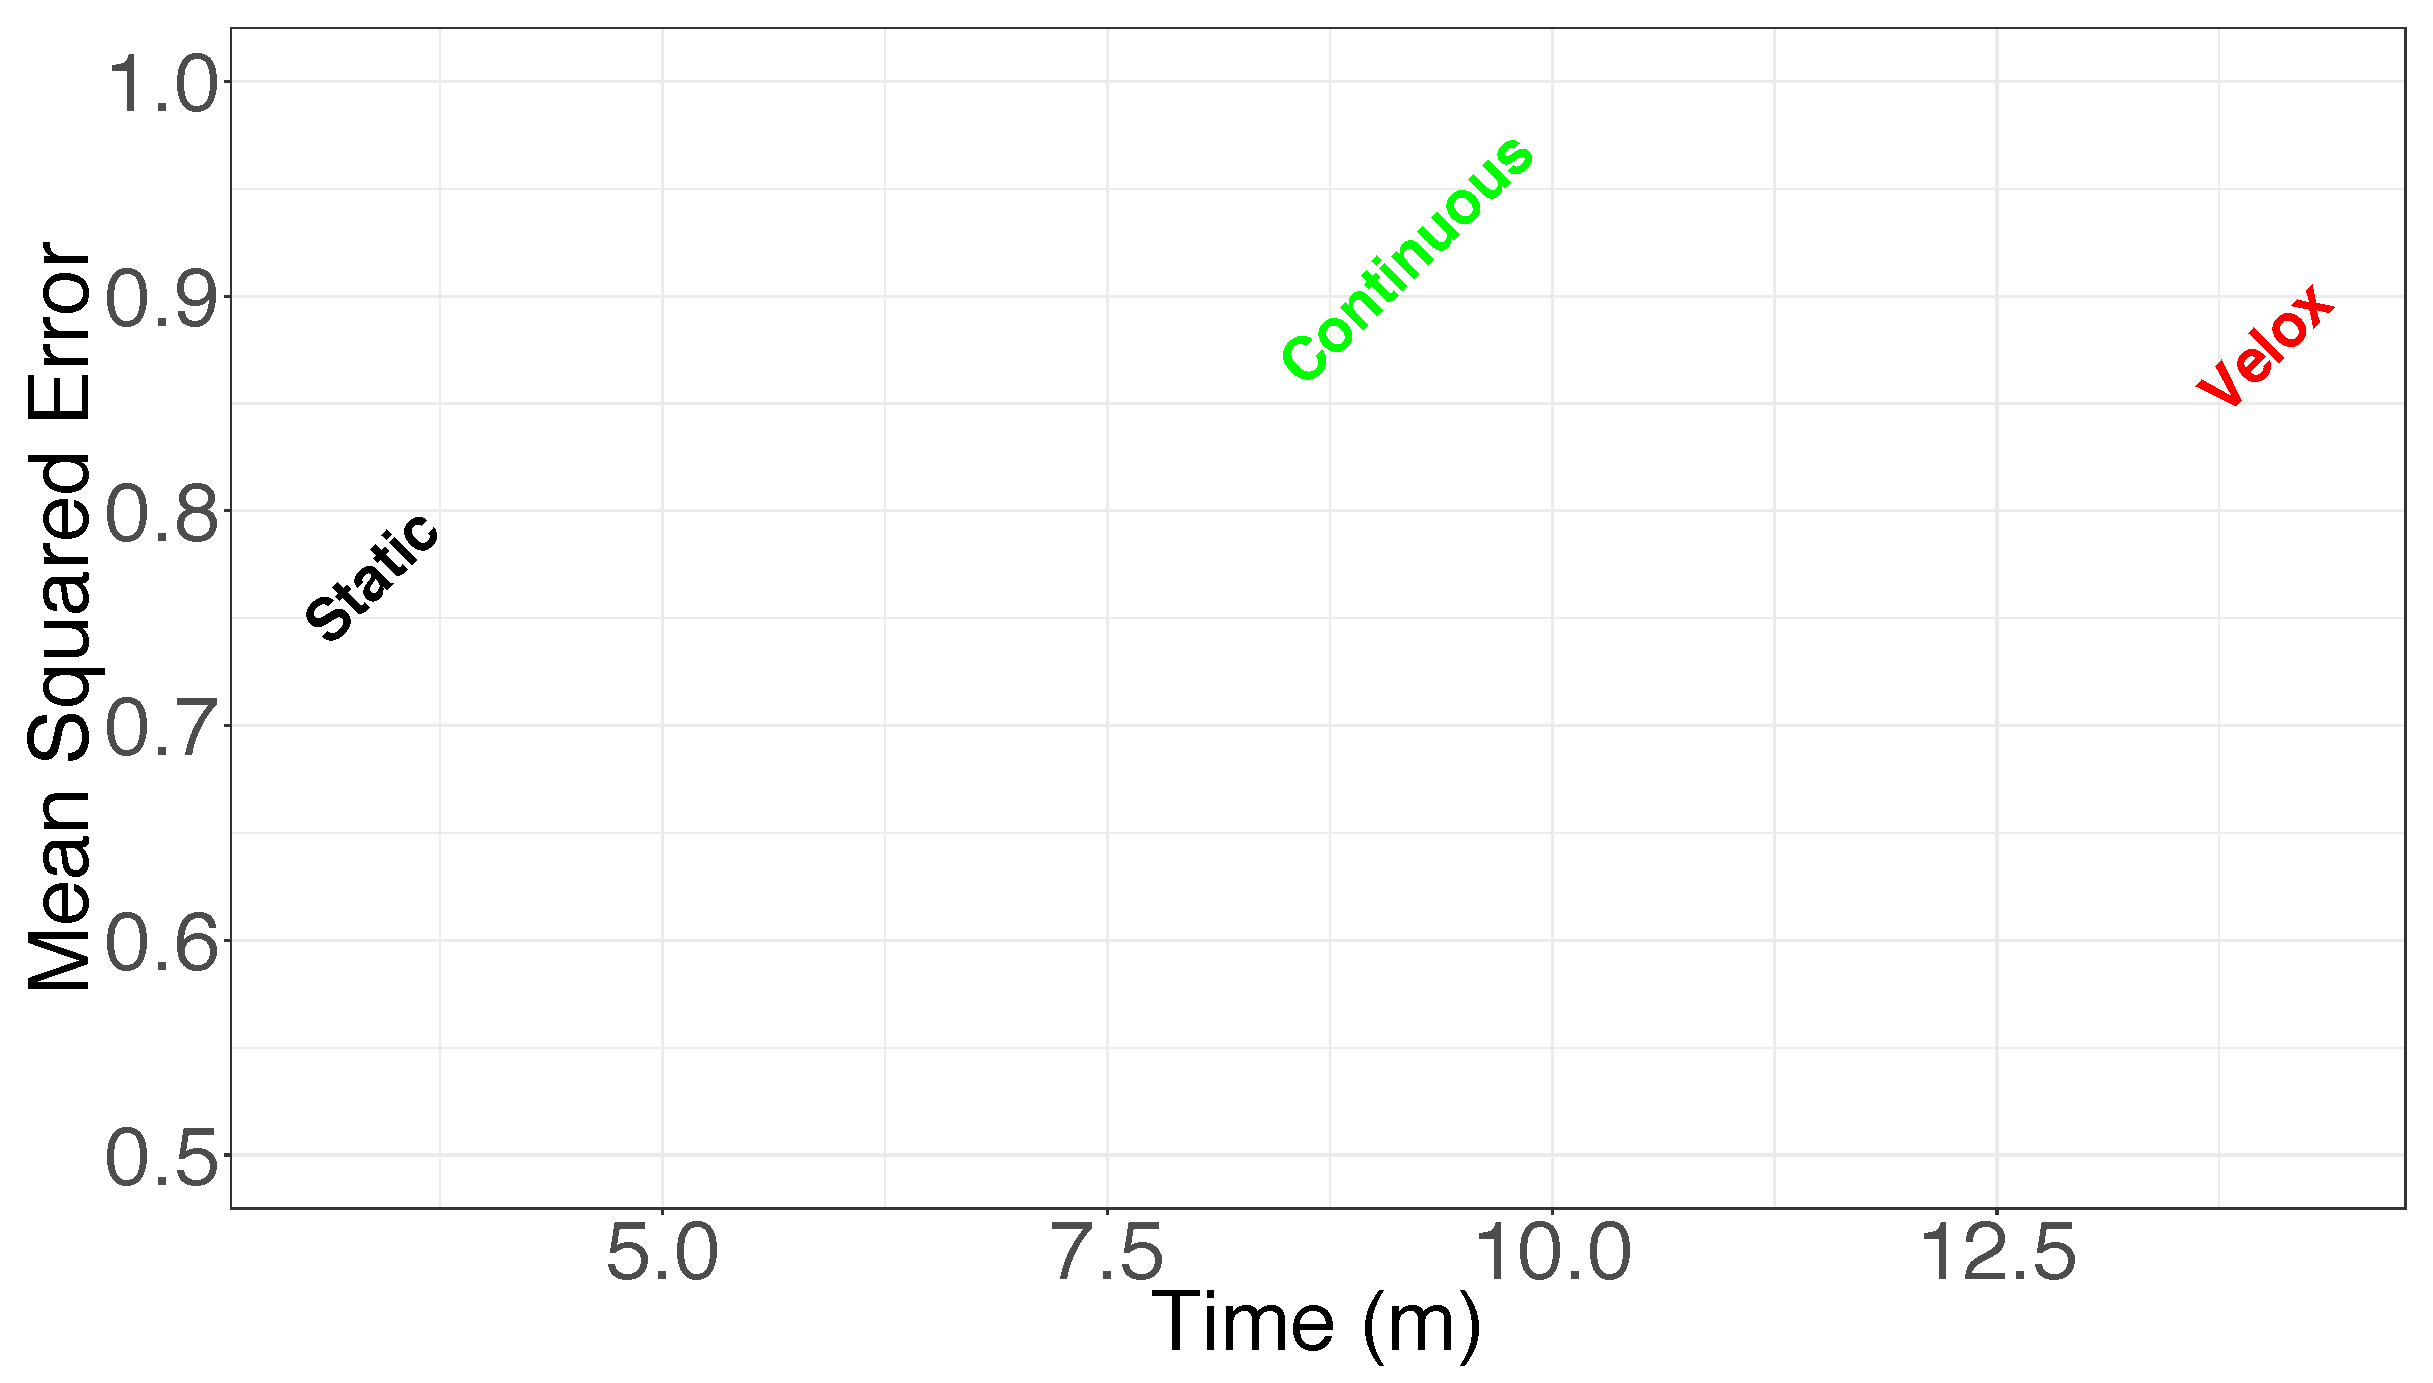
\includegraphics[width=\linewidth]{../images/experiment-results/movie-lens-100k-systems.eps}
  \caption{Movie Lens 100K}
  \label{fig:sfig2}
\end{subfigure}%
\begin{subfigure}{0.5\textwidth}
  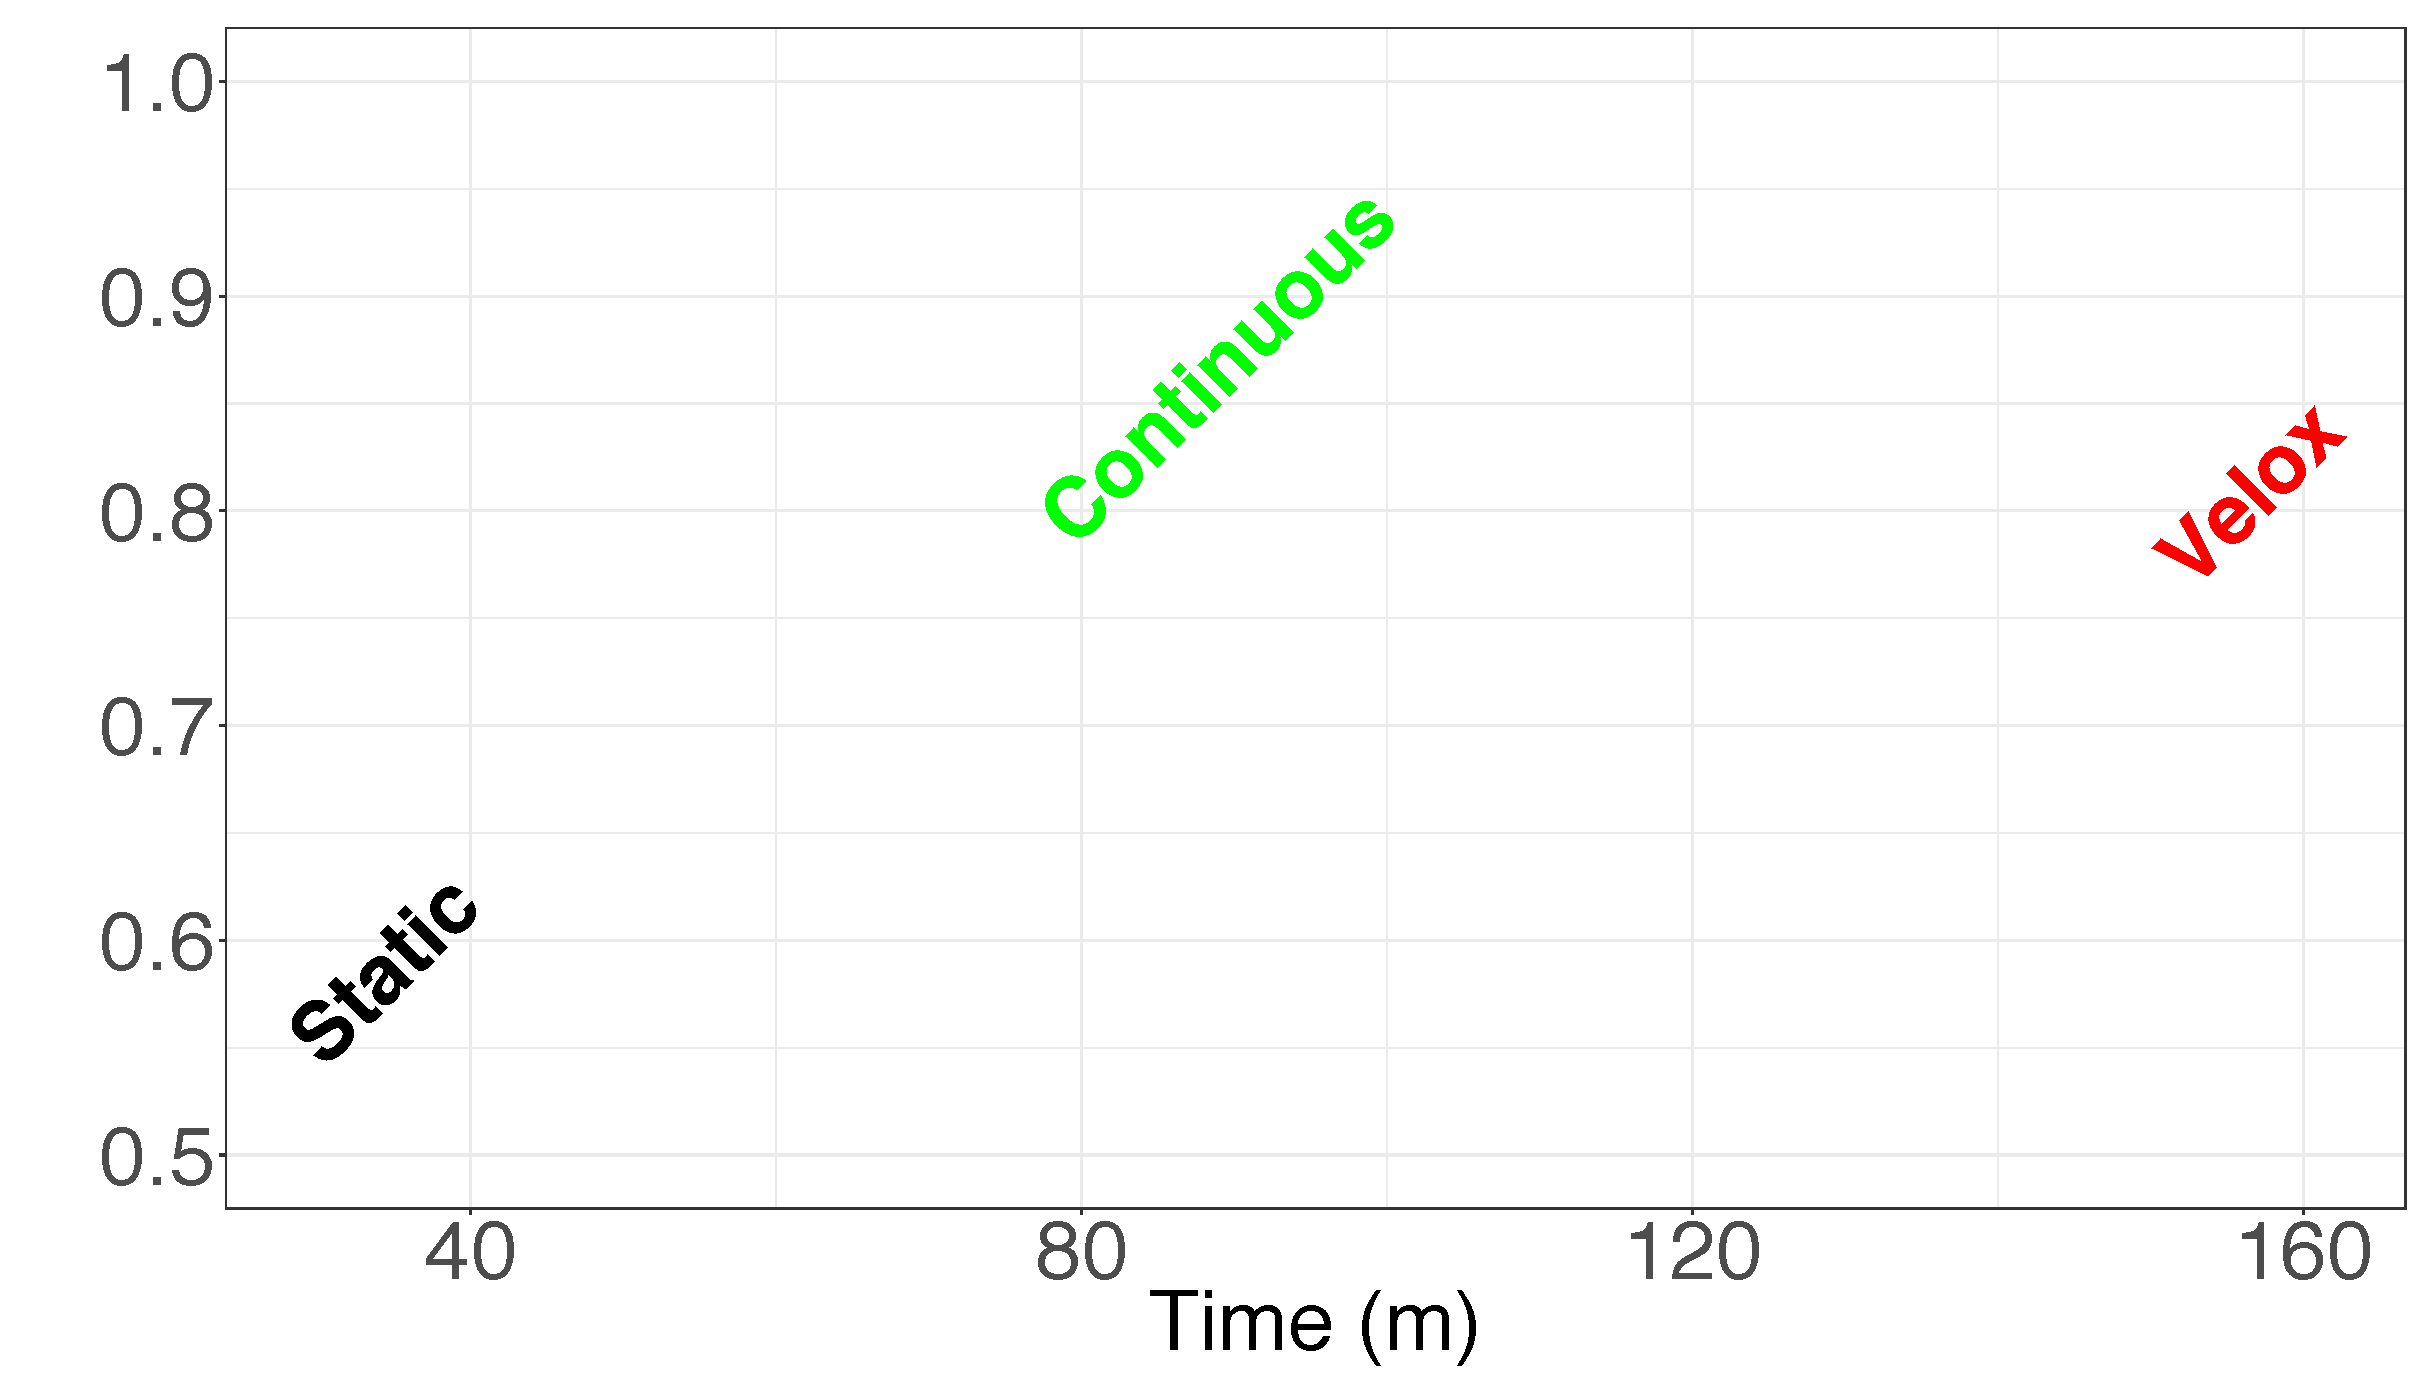
\includegraphics[width=\linewidth]{../images/experiment-results/movie-lens-1m-systems.eps}
  \caption{Movie Lens 1M}
  \label{fig:sfig1}
\end{subfigure}

\caption{Performance vs Quality}
\label{fig:fig}
\end{figure*}

\section{Related Work} \label{related-work}
\begin{figure*}[!t]
\centering
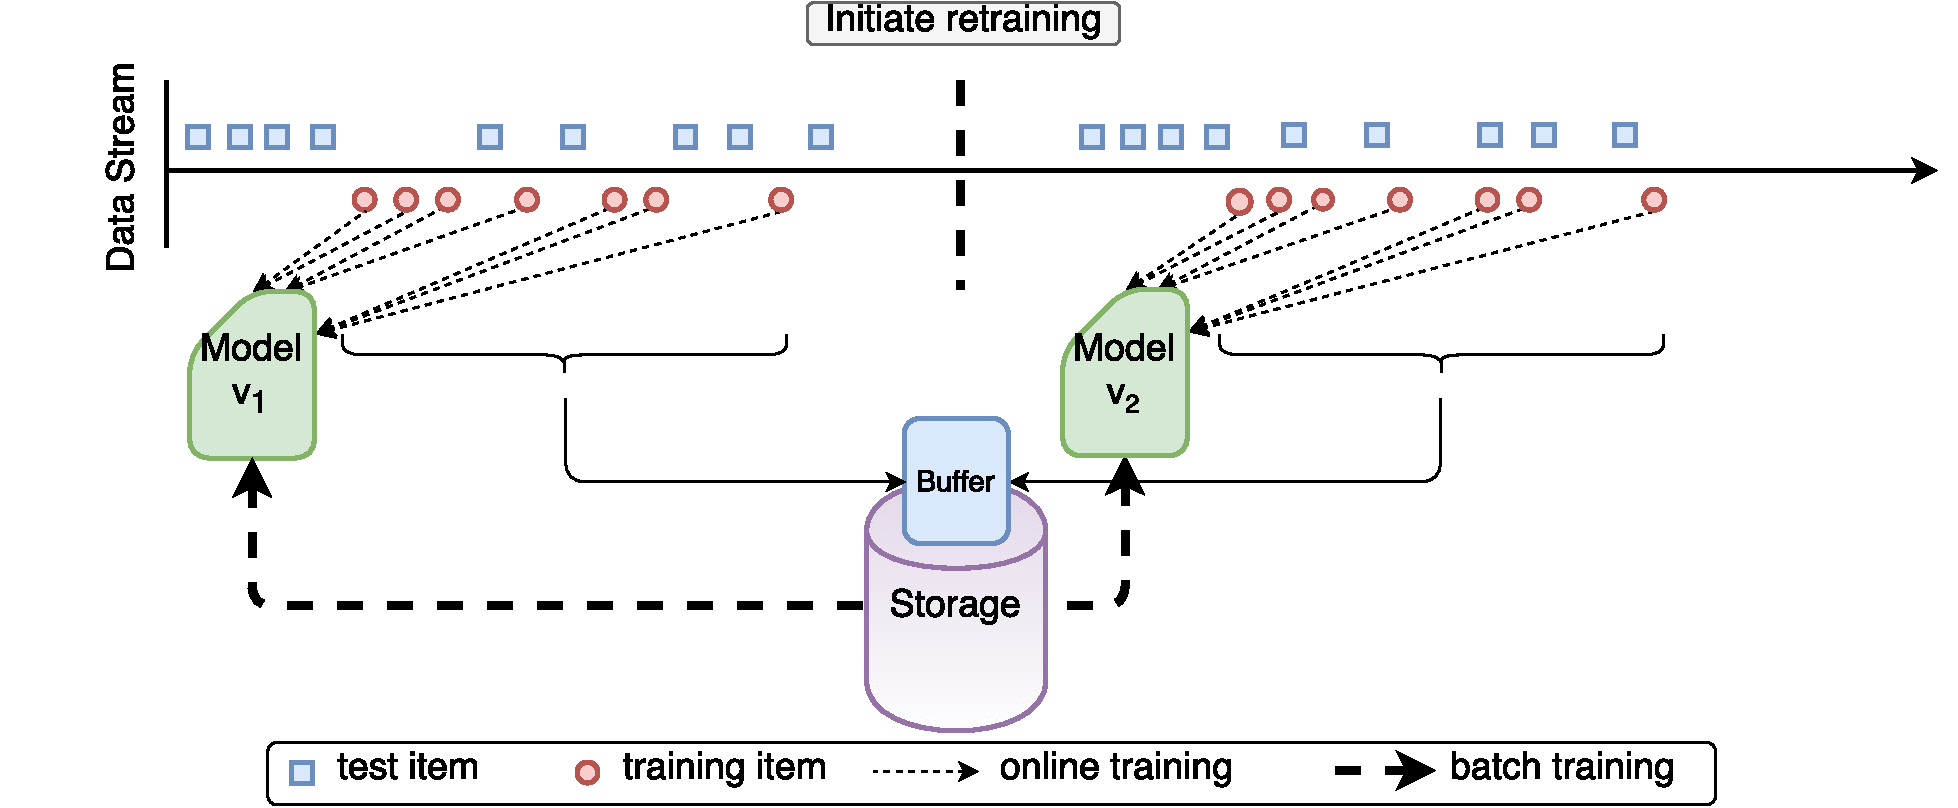
\includegraphics[scale = 0.5]{../images/velox-1.pdf}
\caption{Velox Work Flow}
\label{fig:velox-work-flow}
\end{figure*}
Traditional machine learning systems focus on training and management of models and leave the task of deployment and maintenance to the users. 
It has only been recently that some systems, for example Velox \cite{crankshaw2014missing}, TensorFlow Serving \cite{abadi2016tensorflow}, and LongView \cite{akdere2011case} have proposed architectures to support model deployment and query answering as well. 
LongView integrates predictive machine learning models into relational databases. 
It answers predictive queries and maintains and manages the models.
LongView uses techniques such as query optimization and materialized view selection to increase the performance of the system.
However, LongView only works with batch data and does not provide support for realtime queries. 
As a result it does not support incremental learning neither.
Our system supports both realtime and incremental learning.
TensorFlow Serving provides mechanisms for realtime queries, deployment and version control of machine learning models.
It has out-of-the-box support for models created using TensorFlow and it provides several interfaces for users to deploy their custom models.
However, it does not provide incremental updates to the model.
Contrary to our system, models have to be retrained outside of the system and redeployed to TensorFlow Serving once the training is done.
Our system supports, incremental and batch updates to the model and automatically applies these updates to the model currently being served.
\todo[inline]{FIX THIS}
Velox \cite{crankshaw2014missing} is an state of the art system which has implemented this deployment model.
It uses Apache Spark to train an initial model using the available training data.
Once the model is trained, it is deployed into a distributed environment, where prediction queries are answered in real time.
When new training data arrives at the system the model is incrementally updated.
The incoming training data is also stored in a persistent storage.
To ensure the model is performing well, its quality is monitored over time.
Velox periodically retrains the model from scratch. 
This retraining can be triggered when the size of new training data has surpasses a predefined limit, or the quality of the model has gone below a user defined threshold or simply after a fixed period of time defined by the user.
Figure \ref{fig:velox-work-flow} depicts how Velox works. 
A buffer is used to store the incoming training observations, which will be combined with the historical data during the next retraining phase.
Although Velox continuously monitors and updates the underlying model, it has 3 drawbacks:\\
\begin{itemize}
\item Complete retraining discards all the current model parameter
\item Process of retraining on full dataset is a time consuming process that requires a lot of resources
\item When new datasets are introduced, a complete retraining has to be performed in order to update the model
\end{itemize}
While the model is being retrained, incremental updates are turned off.
Moreover, newly introduced datasets will not have any effect on the model until the next retraining.
This negatively affects the quality of the predictions produced by the system.
To address these problems, we introduced a new deployment system which we describe next.

Velox \cite{crankshaw2014missing} is an implementation of the common machine learning serving practice, explained in section \ref{introduction}.
Velox supports incremental learning and can answer prediction queries in realtime.
It also eliminates the need for users to manually retrain the model offline and redeploy it again.
Velox monitors the quality of the model using a validation set and once the error rate has gone beyond a predefined threshold it initiates a complete retraining of the model using Spark. 
This deployment method, however, has three drawbacks; retraining discards updates that have been applied to the model so far, the process of retraining on full data set is resource intensive and time consuming and new datasets introduced to the system only influence the model after the next retraining.
Our system uses the underlying properties of SGD to fully integrate the training process into the system's lifeline and eliminate the need for complete retraining of the model, which both reduces the time spent on training and can produce an updated model swiftly.
Clipper \cite{crankshaw2016clipper} is another machine learning deployment system that focuses on producing higher quality predictions by maintaining an ensemble of models.
It constantly examines the confidence of each model and for each prediction request, it uses the model with the highest confidence.
However, it does not incrementally train the models in production which overtime leads to models becoming outdated.
Our deployment model on the other hand, focuses on maintenance and constant updates of the models in production environment.

Weka \cite{hall2009weka}, Apache Mahout \cite{Owen:2011:MA:2132656}, and Madlib \cite{hellerstein2012madlib} are systems that provide the necessary toolkits to train machine learning models. All of these systems provide a range of machine learning training algorithms. 
They, however, do not provide any management, before or after deployment of these models. 
Our proposed system focuses on models trainable using Stochastic Gradient Descent and as a result is able to provide management of the models both in training and after deployment.

MLBase \cite{kraska2013mlbase} and TuPaq \cite{sparks2015tupaq} are machine learning model management systems.
They provide a range of training algorithms to create machine learning models and mechanism for model search as well as model management.
However, once models are created, they have to be deployed and used for serving manually by the users.
Our system, on the contrary, is designed for deployment and maintenance of already trained models.

\section{Conclusions} \label{conclusion}
This paper presents an architecture for deployment and continuous training of machine learning models.
The architecture utilizes the properties of stochastic gradient descent optimization method.
SGD is an iterative optimization process where in each iteration a small sample of the data is used to update the machine learning model, however, it typically works with static datasets.
Our proposed architecture uses the properties of the SGD and applies it to long running, integrated training and deployment processes.
Every successive iteration of SGD is scheduled to run while the machine learning model is being used to answer prediction queries.
After every iteration, the model is updated with the new parameters.
SGD is one of the most common optimization techniques for large datasets and has been successfully used in different domains such as neural networks, recommender systems, regression, and clustering models. This makes our architecture applicable for a large range of machine learning models beyond the ones demonstrated in the evaluation.

%new paragraph
To demonstrate our system's ability to incorporate different machine learning models and workloads, we implement two use cases: recommender system and Image classifier.
The recommender system is tested on different workloads and the results show that not only it scales well but also it adopts to changes in data distribution by continuously updating the model.
Image classifier use case as well shows how we can implement and use neural networks within our system to create a model that not only can answer prediction requests quickly, but is also able to make incremental and batch updates to further increase the model quality without creating much overhead.
% end of new paragraph
Our experiments also shows the continuous training of the machine learning models is much faster than full retraining of them, which is the most common approach in deployment and maintenance of machine learning models. We showed that not only continuous training requires less resources but it also produces models with lower error rates that adopt faster to changes in the dataset.
Moreover, comparing to simple techniques such incremental learning or initial batch training it produces a model with higher quality.

In future work, we will explore other optimization strategies such as batching of prediction queries, caching of query results, and more advanced methods for sampling of historical data in order to investigate their effect on the performance of the system.
%ACKNOWLEDGMENTS are optional
%\section{Acknowledgments}
\bibliographystyle{plain}
\bibliography{main}
\end{document}